% This file is part of GUFI, which is part of MarFS, which is released
% under the BSD license.
%
%
% Copyright (c) 2017, Los Alamos National Security (LANS), LLC
% All rights reserved.
%
% Redistribution and use in source and binary forms, with or without modification,
% are permitted provided that the following conditions are met:
%
% 1. Redistributions of source code must retain the above copyright notice, this
% list of conditions and the following disclaimer.
%
% 2. Redistributions in binary form must reproduce the above copyright notice,
% this list of conditions and the following disclaimer in the documentation and/or
% other materials provided with the distribution.
%
% 3. Neither the name of the copyright holder nor the names of its contributors
% may be used to endorse or promote products derived from this software without
% specific prior written permission.
%
% THIS SOFTWARE IS PROVIDED BY THE COPYRIGHT HOLDERS AND CONTRIBUTORS "AS IS" AND
% ANY EXPRESS OR IMPLIED WARRANTIES, INCLUDING, BUT NOT LIMITED TO, THE IMPLIED
% WARRANTIES OF MERCHANTABILITY AND FITNESS FOR A PARTICULAR PURPOSE ARE DISCLAIMED.
% IN NO EVENT SHALL THE COPYRIGHT HOLDER OR CONTRIBUTORS BE LIABLE FOR ANY DIRECT,
% INDIRECT, INCIDENTAL, SPECIAL, EXEMPLARY, OR CONSEQUENTIAL DAMAGES (INCLUDING,
% BUT NOT LIMITED TO, PROCUREMENT OF SUBSTITUTE GOODS OR SERVICES; LOSS OF USE,
% DATA, OR PROFITS; OR BUSINESS INTERRUPTION) HOWEVER CAUSED AND ON ANY THEORY OF
% LIABILITY, WHETHER IN CONTRACT, STRICT LIABILITY, OR TORT (INCLUDING NEGLIGENCE
% OR OTHERWISE) ARISING IN ANY WAY OUT OF THE USE OF THIS SOFTWARE, EVEN IF
% ADVISED OF THE POSSIBILITY OF SUCH DAMAGE.
%
%
% From Los Alamos National Security, LLC:
% LA-CC-15-039
%
% Copyright (c) 2017, Los Alamos National Security, LLC All rights reserved.
% Copyright 2017. Los Alamos National Security, LLC. This software was produced
% under U.S. Government contract DE-AC52-06NA25396 for Los Alamos National
% Laboratory (LANL), which is operated by Los Alamos National Security, LLC for
% the U.S. Department of Energy. The U.S. Government has rights to use,
% reproduce, and distribute this software.  NEITHER THE GOVERNMENT NOR LOS
% ALAMOS NATIONAL SECURITY, LLC MAKES ANY WARRANTY, EXPRESS OR IMPLIED, OR
% ASSUMES ANY LIABILITY FOR THE USE OF THIS SOFTWARE.  If software is
% modified to produce derivative works, such modified software should be
% clearly marked, so as not to confuse it with the version available from
% LANL.
%
% THIS SOFTWARE IS PROVIDED BY LOS ALAMOS NATIONAL SECURITY, LLC AND CONTRIBUTORS
% "AS IS" AND ANY EXPRESS OR IMPLIED WARRANTIES, INCLUDING, BUT NOT LIMITED TO,
% THE IMPLIED WARRANTIES OF MERCHANTABILITY AND FITNESS FOR A PARTICULAR PURPOSE
% ARE DISCLAIMED. IN NO EVENT SHALL LOS ALAMOS NATIONAL SECURITY, LLC OR
% CONTRIBUTORS BE LIABLE FOR ANY DIRECT, INDIRECT, INCIDENTAL, SPECIAL,
% EXEMPLARY, OR CONSEQUENTIAL DAMAGES (INCLUDING, BUT NOT LIMITED TO, PROCUREMENT
% OF SUBSTITUTE GOODS OR SERVICES; LOSS OF USE, DATA, OR PROFITS; OR BUSINESS
% INTERRUPTION) HOWEVER CAUSED AND ON ANY THEORY OF LIABILITY, WHETHER IN
% CONTRACT, STRICT LIABILITY, OR TORT (INCLUDING NEGLIGENCE OR OTHERWISE) ARISING
% IN ANY WAY OUT OF THE USE OF THIS SOFTWARE, EVEN IF ADVISED OF THE POSSIBILITY
% OF SUCH DAMAGE.



\documentclass{article}

% Useful packages
\usepackage{fixltx2e}
\usepackage{float}
\usepackage{graphicx}
\usepackage{hyperref}
\usepackage{longtable}
\usepackage{rotating}
\usepackage{tabularx}
\usepackage{tikz}
\usepackage{verbatim}
\usepackage{GUFIText}

\hypersetup{
    colorlinks,
    citecolor=black,
    filecolor=black,
    linkcolor=black,
    urlcolor=blue
}

\usetikzlibrary{positioning}

\setcounter{tocdepth}{4}
\setcounter{secnumdepth}{4}

\title{GUFI Developer's Guide}
\author{GUFI Developers}

\begin{document}

\maketitle

\tableofcontents
\include{sections/license}
\include{sections/introduction}
\include{sections/requirements}
\include{sections/design}
% This file is part of GUFI, which is part of MarFS, which is released
% under the BSD license.
%
%
% Copyright (c) 2017, Los Alamos National Security (LANS), LLC
% All rights reserved.
%
% Redistribution and use in source and binary forms, with or without modification,
% are permitted provided that the following conditions are met:
%
% 1. Redistributions of source code must retain the above copyright notice, this
% list of conditions and the following disclaimer.
%
% 2. Redistributions in binary form must reproduce the above copyright notice,
% this list of conditions and the following disclaimer in the documentation and/or
% other materials provided with the distribution.
%
% 3. Neither the name of the copyright holder nor the names of its contributors
% may be used to endorse or promote products derived from this software without
% specific prior written permission.
%
% THIS SOFTWARE IS PROVIDED BY THE COPYRIGHT HOLDERS AND CONTRIBUTORS "AS IS" AND
% ANY EXPRESS OR IMPLIED WARRANTIES, INCLUDING, BUT NOT LIMITED TO, THE IMPLIED
% WARRANTIES OF MERCHANTABILITY AND FITNESS FOR A PARTICULAR PURPOSE ARE DISCLAIMED.
% IN NO EVENT SHALL THE COPYRIGHT HOLDER OR CONTRIBUTORS BE LIABLE FOR ANY DIRECT,
% INDIRECT, INCIDENTAL, SPECIAL, EXEMPLARY, OR CONSEQUENTIAL DAMAGES (INCLUDING,
% BUT NOT LIMITED TO, PROCUREMENT OF SUBSTITUTE GOODS OR SERVICES; LOSS OF USE,
% DATA, OR PROFITS; OR BUSINESS INTERRUPTION) HOWEVER CAUSED AND ON ANY THEORY OF
% LIABILITY, WHETHER IN CONTRACT, STRICT LIABILITY, OR TORT (INCLUDING NEGLIGENCE
% OR OTHERWISE) ARISING IN ANY WAY OUT OF THE USE OF THIS SOFTWARE, EVEN IF
% ADVISED OF THE POSSIBILITY OF SUCH DAMAGE.
%
%
% From Los Alamos National Security, LLC:
% LA-CC-15-039
%
% Copyright (c) 2017, Los Alamos National Security, LLC All rights reserved.
% Copyright 2017. Los Alamos National Security, LLC. This software was produced
% under U.S. Government contract DE-AC52-06NA25396 for Los Alamos National
% Laboratory (LANL), which is operated by Los Alamos National Security, LLC for
% the U.S. Department of Energy. The U.S. Government has rights to use,
% reproduce, and distribute this software.  NEITHER THE GOVERNMENT NOR LOS
% ALAMOS NATIONAL SECURITY, LLC MAKES ANY WARRANTY, EXPRESS OR IMPLIED, OR
% ASSUMES ANY LIABILITY FOR THE USE OF THIS SOFTWARE.  If software is
% modified to produce derivative works, such modified software should be
% clearly marked, so as not to confuse it with the version available from
% LANL.
%
% THIS SOFTWARE IS PROVIDED BY LOS ALAMOS NATIONAL SECURITY, LLC AND CONTRIBUTORS
% "AS IS" AND ANY EXPRESS OR IMPLIED WARRANTIES, INCLUDING, BUT NOT LIMITED TO,
% THE IMPLIED WARRANTIES OF MERCHANTABILITY AND FITNESS FOR A PARTICULAR PURPOSE
% ARE DISCLAIMED. IN NO EVENT SHALL LOS ALAMOS NATIONAL SECURITY, LLC OR
% CONTRIBUTORS BE LIABLE FOR ANY DIRECT, INDIRECT, INCIDENTAL, SPECIAL,
% EXEMPLARY, OR CONSEQUENTIAL DAMAGES (INCLUDING, BUT NOT LIMITED TO, PROCUREMENT
% OF SUBSTITUTE GOODS OR SERVICES; LOSS OF USE, DATA, OR PROFITS; OR BUSINESS
% INTERRUPTION) HOWEVER CAUSED AND ON ANY THEORY OF LIABILITY, WHETHER IN
% CONTRACT, STRICT LIABILITY, OR TORT (INCLUDING NEGLIGENCE OR OTHERWISE) ARISING
% IN ANY WAY OUT OF THE USE OF THIS SOFTWARE, EVEN IF ADVISED OF THE POSSIBILITY
% OF SUCH DAMAGE.



\section{Dependencies}
A number of dependencies that should be installed before attempting to
build GUFI. There are also many optional dependencies that can enable
optional features.

\subsection{System Tools}
\begin{tabularx}{\textwidth}{| l | c | X | }
  \hline
  Package/Executable & Required? & Comments \\
  \hline
  autotools & Yes & Some bundled packages use autotools \\
  \hline
  C Compiler & Yes & C99 support \\
  \hline
  C++ Compiler & No & C++11 support - g++ 4.9.3, clang++-3.9, or newer
  \hfill \\
  \hline
  CMake & Yes & Version 3.16 or higher \\
  \hline
  column & Yes & \\
  \hline
  Make & Yes & \\
  \hline
  Python & Yes & Python 2.7 or Python 3 \\
  \hline
  pip & No & Used for installing and client dependencies \\
  \hline
  git & No & \\
  \hline
  ImageMagick & No & Only needed if building \LaTeX \hfill \\
  & & Documentation \hfill \\
  \hline
  \LaTeX & No & Only needed if building \LaTeX \hfill \\
  & & Documentation \hfill \\
  \hline
  patch & Yes & \\
  \hline
  pkg-config & Yes & \\
  \hline
  realpath & Yes & \\
  \hline
  rpmbuild & No & Only needed if building RPMs \\
  \hline
  setfattr & Yes & attr package \\
  & & \texttt{xattr -w} on OSX \\
  \hline
  truncate & Yes & The -s option must be available \\
  \hline
  uname & No & Only needed if building RPMs \\
  \hline
\end{tabularx}

\subsection{Libraries}
\begin{tabularx}{\textwidth}{| l | c | X |}
  \hline
  Name & Required? & Comments \\
  \hline
  xattr & Yes & \\
  \hline
  pcre & Yes & Version 2 compiled with \texttt{-fPIC} \\
  \hline
  fuse & No & Called osxfuse on OSX. Not updating to macfuse for now
  because pkg-config can't seem to find it. \\
  \hline
  db2 & No & \\
  \hline
  gpfs & No & \\
  \hline
  zlib & No & \\
  \hline
\end{tabularx}

\subsection{Packages provided by GUFI}
Several packages are provided/downloaded, built, and installed
automatically:
\begin{tabularx}{\textwidth}{| l | X |}
  \hline
  Name & Comments \\
  \hline
  GoogleTest & \url{https://github.com/google/googletest} \\
  \hline
  jemalloc & \url{https://github.com/jemalloc/jemalloc} \\
  \hline
  sqlite3 & \url{https://www.sqlite.org/index.html} \\
  & patched sqlite-autoconf-3430100.tar.gz \\
  \hline
  sqlite3-pcre & \url{https://github.com/mar-file-system/sqlite3-pcre/tree/pcre2}
  \\
  \hline
\end{tabularx}

% This file is part of GUFI, which is part of MarFS, which is released
% under the BSD license.
%
%
% Copyright (c) 2017, Los Alamos National Security (LANS), LLC
% All rights reserved.
%
% Redistribution and use in source and binary forms, with or without modification,
% are permitted provided that the following conditions are met:
%
% 1. Redistributions of source code must retain the above copyright notice, this
% list of conditions and the following disclaimer.
%
% 2. Redistributions in binary form must reproduce the above copyright notice,
% this list of conditions and the following disclaimer in the documentation and/or
% other materials provided with the distribution.
%
% 3. Neither the name of the copyright holder nor the names of its contributors
% may be used to endorse or promote products derived from this software without
% specific prior written permission.
%
% THIS SOFTWARE IS PROVIDED BY THE COPYRIGHT HOLDERS AND CONTRIBUTORS "AS IS" AND
% ANY EXPRESS OR IMPLIED WARRANTIES, INCLUDING, BUT NOT LIMITED TO, THE IMPLIED
% WARRANTIES OF MERCHANTABILITY AND FITNESS FOR A PARTICULAR PURPOSE ARE DISCLAIMED.
% IN NO EVENT SHALL THE COPYRIGHT HOLDER OR CONTRIBUTORS BE LIABLE FOR ANY DIRECT,
% INDIRECT, INCIDENTAL, SPECIAL, EXEMPLARY, OR CONSEQUENTIAL DAMAGES (INCLUDING,
% BUT NOT LIMITED TO, PROCUREMENT OF SUBSTITUTE GOODS OR SERVICES; LOSS OF USE,
% DATA, OR PROFITS; OR BUSINESS INTERRUPTION) HOWEVER CAUSED AND ON ANY THEORY OF
% LIABILITY, WHETHER IN CONTRACT, STRICT LIABILITY, OR TORT (INCLUDING NEGLIGENCE
% OR OTHERWISE) ARISING IN ANY WAY OUT OF THE USE OF THIS SOFTWARE, EVEN IF
% ADVISED OF THE POSSIBILITY OF SUCH DAMAGE.
%
%
% From Los Alamos National Security, LLC:
% LA-CC-15-039
%
% Copyright (c) 2017, Los Alamos National Security, LLC All rights reserved.
% Copyright 2017. Los Alamos National Security, LLC. This software was produced
% under U.S. Government contract DE-AC52-06NA25396 for Los Alamos National
% Laboratory (LANL), which is operated by Los Alamos National Security, LLC for
% the U.S. Department of Energy. The U.S. Government has rights to use,
% reproduce, and distribute this software.  NEITHER THE GOVERNMENT NOR LOS
% ALAMOS NATIONAL SECURITY, LLC MAKES ANY WARRANTY, EXPRESS OR IMPLIED, OR
% ASSUMES ANY LIABILITY FOR THE USE OF THIS SOFTWARE.  If software is
% modified to produce derivative works, such modified software should be
% clearly marked, so as not to confuse it with the version available from
% LANL.
%
% THIS SOFTWARE IS PROVIDED BY LOS ALAMOS NATIONAL SECURITY, LLC AND CONTRIBUTORS
% "AS IS" AND ANY EXPRESS OR IMPLIED WARRANTIES, INCLUDING, BUT NOT LIMITED TO,
% THE IMPLIED WARRANTIES OF MERCHANTABILITY AND FITNESS FOR A PARTICULAR PURPOSE
% ARE DISCLAIMED. IN NO EVENT SHALL LOS ALAMOS NATIONAL SECURITY, LLC OR
% CONTRIBUTORS BE LIABLE FOR ANY DIRECT, INDIRECT, INCIDENTAL, SPECIAL,
% EXEMPLARY, OR CONSEQUENTIAL DAMAGES (INCLUDING, BUT NOT LIMITED TO, PROCUREMENT
% OF SUBSTITUTE GOODS OR SERVICES; LOSS OF USE, DATA, OR PROFITS; OR BUSINESS
% INTERRUPTION) HOWEVER CAUSED AND ON ANY THEORY OF LIABILITY, WHETHER IN
% CONTRACT, STRICT LIABILITY, OR TORT (INCLUDING NEGLIGENCE OR OTHERWISE) ARISING
% IN ANY WAY OUT OF THE USE OF THIS SOFTWARE, EVEN IF ADVISED OF THE POSSIBILITY
% OF SUCH DAMAGE.



\section{Build}

GUFI uses CMake to generate Makefiles. CMake 3.19 or higher is
required. From the root directory of the GUFI source, run:
\begin{verbatim}
mkdir build
cd build
cmake .. [options]
make
\end{verbatim}

The recommended options for deployment are
\texttt{-DCMAKE\_BUILD\_TYPE=Release -DCLIENT=On}.
\\\\
The list below shows the environments where GUFI is known to have
built, run, and passed tests at some point. The environments labeled
with a plus (+) are currently being used on Github Actions. The
environments labeled with minus (-) are no longer used on GitHub
Actions and might no longer work.
\begin{itemize}
\item Linux
  \begin{itemize}
  \item[+] Alpine~Linux~Edge
  \item[-] CentOS~7
  \item[+] CentOS~8
  \item[-] OpenSUSE~12.3
  \item[-] Ubuntu~16.04~(Xenial)
  \item[-] Ubuntu~18.04~(Bionic)
  \item[-] Ubuntu~20.04~(Focal)
  \item[+] Ubuntu~22.04~(Jammy)
  \item[+] Ubuntu~24.04~(Noble)
  \item[+] Rocky~Linux~8
  \item[+] Rocky~Linux~9
  \end{itemize}
\item macOS
  \begin{itemize}
  \item[-] 10.13~(High~Sierra)
  \item[-] 11~(Big~Sur)
  \item[-] 12~(Monterey)
  \item[-] 13~(Ventura)
  \item[+] 14~(Sonoma)
  \item[+] 15~(Sequoia)
  \end{itemize}
\item Windows
  \begin{itemize}
  \item[+] cygwin
    \begin{itemize}
    \item GCC (not MinGW)
    \item jemalloc turned off
    \end{itemize}
  \end{itemize}
\end{itemize}

\subsection{Environment Variables}
\begin{table}[h!]
\centering
\begin{tabularx}{1.2\textwidth}{| l | X |}
  \hline
  Setting & Description \\
  \hline
  \texttt{CXX=false} & Disable building of C++ code \\
  \hline
\end{tabularx}
\end{table}

\subsection{CMake Flags}

\subsubsection{General}
\begin{table}[h!]
\centering
\begin{tabularx}{1.2\textwidth}{| l | X |}
  \hline
  \texttt{-D<VAR>=<VALUE>} & Description \\
  \hline
  \texttt{CMAKE\_INSTALL\_PREFIX=<PATH>}
  & Install to a custom directory when running \texttt{make install} \\
  \hline
  \texttt{CMAKE\_BUILD\_TYPE=Debug}
  & Build with warnings and debugging symbols turned on \\
  \hline
\end{tabularx}
\end{table}

\subsubsection{Dependencies}
\begin{table}[H] % do not change
\centering
\begin{tabularx}{1.2\textwidth}{| l | X |}
  \hline
  \texttt{-D<VAR>=<VALUE>} & Description \\
  \hline
  \texttt{DEP\_AI=<On|Off>}
  & Whether or not to build with \sqlite AI modules (default: On) \\
  \hline
  \texttt{DEP\_DOWNLOAD\_PREFIX=<PATH>}
  & Location of downloaded dependencies. If the expected files are
  found, they will not be downloaded. The default path points to the
  bundled dependencies. \\
  \hline
  \texttt{DEP\_BUILD\_DIR\_PREFIX=<PATH>}
  & Location to build dependencies. Defaults to \\
  & \$\{CMAKE\_BINARY\_DIR\}/builds \\
  \hline
  \texttt{DEP\_INSTALL\_PREFIX=<PATH>}
  & Location to install the dependencies. Defaults to
  \$\{CMAKE\_BINARY\_DIR\}/deps. If the dependencies are not
  installed in \$\{CMAKE\_BINARY\_DIR\}, they will not need to be
  redownloaded, rebuilt, or reinstalled everytime \$\{CMAKE\_BINARY\_DIR\}
  is deleted. \\
  \hline
  \texttt{DEP\_PATCH\_SQLITE3\_OPEN=<On|Off>}
  & Whether or not to patch \sqlite open (default: Off) \\
  \hline
  \texttt{DEP\_USE\_JEMALLOC=<On|Off>}
  & Whether or not to build and link with jemalloc (default: On) \\
  \hline
\end{tabularx}
\end{table}

\subsubsection{Debug}
\texttt{CMAKE\_BUILD\_TYPE} must be set to \texttt{Debug} for these to
have effect.

\begin{table}[H]
\centering
\begin{tabularx}{1.2\textwidth}{| l | X |}
  \hline
  \texttt{-D<VAR>=<VALUE>} & Description \\
  \hline
  \texttt{GPROF=<On|Off>}
  & Compile with the \texttt{-pg} flag (default: Off) \\
  \hline
  \texttt{GCOV=<On|Off>}
  & Compile with the \texttt{--coverage} flag (default: Off) \\
  \hline
\end{tabularx}
\end{table}

\subsubsection{System Paths}
Some files are installed into system paths that are not
\texttt{\$\{CMAKE\_INSTALL\_PREFIX\}/bin} or \texttt{\$\{CMAKE\_INSTALL\_PREFIX\}/lib}.

\begin{table}[H]
\centering
\begin{tabularx}{1.2\textwidth}{| l | X |}
  \hline
  \texttt{-D<VAR>=<VALUE>} & Description \\
  \hline
  \texttt{CONFIG\_CLIENT=<FILEPATH>} & Path of configuration file used by scripts. \\
  \texttt{CONFIG\_SERVER=<FILEPATH>} & \\
                                     & Two different paths are available in case the server and client\\
                                     & deployments place their configuration files at different \\
                                     & locations. \\
                                     & \\
                                     & Both default to \guficonfigfile. \\
                                     & \\
                                     & When \texttt{CLIENT=Off}, \texttt{CONFIG\_SERVER} is used as the location of \\
                                     & the configuration file. \\
                                     & \\
                                     & Note that many paths will conflict with the paths of other \\
                                     & packages if installing GUFI via package. If installing GUFI \\
                                     & with \texttt{make install}, point to a convenient location. \\
  \hline
  \texttt{BASH\_COMPLETION=<On|Off>} & Whether or not to install bash completion script to \\
                                     & \texttt{/etc/bash\_completion.d} (default: On). \\
                                     & Useful when running \texttt{make install} without root.\\
  \hline
\end{tabularx}
\end{table}

\subsubsection{Features}
\begin{table}[H]
\centering
\begin{tabularx}{1.2\textwidth}{| l | X |}
  \hline
  \texttt{-D<VAR>=<VALUE>} & Description \\
  \hline
  \texttt{CLIENT=<On|Off>}
  & Whether or not to install \guficlient wrapper scripts when running
  \texttt{make install} and build separate server and client RPMs
  (default: Off) \\
  \hline
  \texttt{QPTPOOL\_SWAP=<On|Off>}
  & Whether or not to build QueuePerThreadPool with work swapping
  (default: On) \\
  \hline
\end{tabularx}
\end{table}

\subsubsection{Testing}
\begin{table}[H]
\centering
\begin{tabularx}{1.2\textwidth}{| l | X |}
  \hline
  \texttt{-D<VAR>=<VALUE>} & Description \\
  \hline
  \texttt{ENABLE\_SUDO\_TESTS=<On|Off>}
  & Run tests that require \texttt{sudo} (default: Off) \\
  & Can also force enabling of tests in case CMake Policy
  \texttt{CMP0109} comes up \\
  \hline
  \texttt{TEST\_WORKING\_DIRECTORY=<PATH>}
  & Directory to run tests in. Defaults to \\
  & \texttt{\$\{CMAKE\_BINARY\_DIR\}/test} \\
  \hline
\end{tabularx}
\end{table}

\subsubsection{Docs}
\begin{table}[H]
\centering
\begin{tabularx}{1.2\textwidth}{| l | X |}
  \hline
  \texttt{-D<VAR>=<VALUE>} & Description \\
  \hline
  \texttt{LATEX\_BUILD=<On|Off>}
  & Whether or not to build PDF documentation when \LaTeX is found
  (default: Off) \\
  \hline
\end{tabularx}
\end{table}

% This file is part of GUFI, which is part of MarFS, which is released
% under the BSD license.
%
%
% Copyright (c) 2017, Los Alamos National Security (LANS), LLC
% All rights reserved.
%
% Redistribution and use in source and binary forms, with or without modification,
% are permitted provided that the following conditions are met:
%
% 1. Redistributions of source code must retain the above copyright notice, this
% list of conditions and the following disclaimer.
%
% 2. Redistributions in binary form must reproduce the above copyright notice,
% this list of conditions and the following disclaimer in the documentation and/or
% other materials provided with the distribution.
%
% 3. Neither the name of the copyright holder nor the names of its contributors
% may be used to endorse or promote products derived from this software without
% specific prior written permission.
%
% THIS SOFTWARE IS PROVIDED BY THE COPYRIGHT HOLDERS AND CONTRIBUTORS "AS IS" AND
% ANY EXPRESS OR IMPLIED WARRANTIES, INCLUDING, BUT NOT LIMITED TO, THE IMPLIED
% WARRANTIES OF MERCHANTABILITY AND FITNESS FOR A PARTICULAR PURPOSE ARE DISCLAIMED.
% IN NO EVENT SHALL THE COPYRIGHT HOLDER OR CONTRIBUTORS BE LIABLE FOR ANY DIRECT,
% INDIRECT, INCIDENTAL, SPECIAL, EXEMPLARY, OR CONSEQUENTIAL DAMAGES (INCLUDING,
% BUT NOT LIMITED TO, PROCUREMENT OF SUBSTITUTE GOODS OR SERVICES; LOSS OF USE,
% DATA, OR PROFITS; OR BUSINESS INTERRUPTION) HOWEVER CAUSED AND ON ANY THEORY OF
% LIABILITY, WHETHER IN CONTRACT, STRICT LIABILITY, OR TORT (INCLUDING NEGLIGENCE
% OR OTHERWISE) ARISING IN ANY WAY OUT OF THE USE OF THIS SOFTWARE, EVEN IF
% ADVISED OF THE POSSIBILITY OF SUCH DAMAGE.
%
%
% From Los Alamos National Security, LLC:
% LA-CC-15-039
%
% Copyright (c) 2017, Los Alamos National Security, LLC All rights reserved.
% Copyright 2017. Los Alamos National Security, LLC. This software was produced
% under U.S. Government contract DE-AC52-06NA25396 for Los Alamos National
% Laboratory (LANL), which is operated by Los Alamos National Security, LLC for
% the U.S. Department of Energy. The U.S. Government has rights to use,
% reproduce, and distribute this software.  NEITHER THE GOVERNMENT NOR LOS
% ALAMOS NATIONAL SECURITY, LLC MAKES ANY WARRANTY, EXPRESS OR IMPLIED, OR
% ASSUMES ANY LIABILITY FOR THE USE OF THIS SOFTWARE.  If software is
% modified to produce derivative works, such modified software should be
% clearly marked, so as not to confuse it with the version available from
% LANL.
%
% THIS SOFTWARE IS PROVIDED BY LOS ALAMOS NATIONAL SECURITY, LLC AND CONTRIBUTORS
% "AS IS" AND ANY EXPRESS OR IMPLIED WARRANTIES, INCLUDING, BUT NOT LIMITED TO,
% THE IMPLIED WARRANTIES OF MERCHANTABILITY AND FITNESS FOR A PARTICULAR PURPOSE
% ARE DISCLAIMED. IN NO EVENT SHALL LOS ALAMOS NATIONAL SECURITY, LLC OR
% CONTRIBUTORS BE LIABLE FOR ANY DIRECT, INDIRECT, INCIDENTAL, SPECIAL,
% EXEMPLARY, OR CONSEQUENTIAL DAMAGES (INCLUDING, BUT NOT LIMITED TO, PROCUREMENT
% OF SUBSTITUTE GOODS OR SERVICES; LOSS OF USE, DATA, OR PROFITS; OR BUSINESS
% INTERRUPTION) HOWEVER CAUSED AND ON ANY THEORY OF LIABILITY, WHETHER IN
% CONTRACT, STRICT LIABILITY, OR TORT (INCLUDING NEGLIGENCE OR OTHERWISE) ARISING
% IN ANY WAY OUT OF THE USE OF THIS SOFTWARE, EVEN IF ADVISED OF THE POSSIBILITY
% OF SUCH DAMAGE.


\section{Database Schema}
\label{sec:schema}
GUFI stores extracted metadata in SQLite3 database files. Each
directory contains a database file named db.db that contains a set of
tables and views designed to facilitate efficient querying of
metadata.

\subsection{\entries}
The \entries table contains file and link metadata extracted from the
source filesystem using \lstat, \readlink, and \listxattr. There are
also a few OS specific columns (\texttt{oss*}) that are unused in base
GUFI. Note that the inode column is a string and not an integer as one
might expect. As a general rule, do not query this table directly.

\subsection{Directory \summary}
The directory \summary table contains the metadata of the current
directory. Additionally, it contains columns that summarizes the
\entries table located in the same database file, such as minimum and
maximum file sizes, uids, and gids. These summary columns can be used
to determine whether or not the \entries table needs to be queried at
all. Note that the inode and pinode colums are strings and not
integers as one might expect.

\begin{figure} [h!]
\centering
\includegraphics[width=1.0\textwidth]{images/Database_Schemas.png}
\caption{\label{fig:Database Schema}Database schema}
\end{figure}

\subsection{\pentries}
The original \pentries view was defined as:
\\\\
\texttt{SELECT entries.*, summary.inode AS pinode, summary.pinode AS
  ppinode FROM entries, summary};
\\\\
This was done in order to not store the parent inode of each entry,
which would be the same for every entry.

Users should prefer query the \pentries view over the \entries table
in order to obtain complete sets of data to query on, and should use
\pentries whenever paths are not required.

\subsubsection{\pentriesrollup}
In order to simplify rolling up indexes (see
Section~\ref{sec:rollup}), the \pentries view was modified to also
union with the \pentriesrollup table, which contains all child
\pentries views copied into the current directory's database file.

\subsection{\vrsummary}
The \vrsummary view is the \summary table with a handful of columns
repeated as aliases. This was done so that the \texttt{rpath} SQL
function can be called to generate the path of a given directory with
the same view and query whether or not the index has been rolled up,
and thus should be preferred over querying the \summary table. Using
the \summary table directly with a rolled up index is possible, but
will complicate queries.

\subsection{\texttt{vrentries}}
The \texttt{vrentries} view does not exist because it would be a
misuse of the schema: the entries table itself is never rolled up, so
querying a \texttt{vr} version of it would result in incorrect output.

\subsection{\vrpentries}
The \vrpentries view is the \pentries view with a few \summary table
columns aliased. This allows for the \texttt{rpath} SQL function can
be called to generate the path of a given directory with the same view
and query whether or not the index has been rolled up, and thus should
be preferred over querying \entries and \pentries. \texttt{rpath} with
the \vrpentries view is called with the same arguments that are used
with \vrsummary. Using the \pentries view directly with a rolled up
index is possible, but will complicate queries.

\subsection{\treesummary}
Similar to the directory \summary table, GUFI also provides
functionality to generate \treesummary tables. Instead of summarizing
only the data found in the entries table of the current directory, the
\treesummary table summarizes the contents of the entire subtree,
allowing for queries to completely skip processing entire
subtrees. See Section~\ref{sec:treesummary} for details.

\subsection{\vsummarydir}
The \vsummarydir view provides access to the entire directory summary
and not a partial directory summary (say by user or group).

\subsection{\vsummaryuser}
The \vsummaryuser view provides access to the directory summary for
each user (if this summary has been populated (not by default but
easily populatable via a query)).

\subsection{\vsummarygroup}
The \vsummarygroup view provides access to the directory summary for
each group (if this summary row has been created (not by default but
easily created via a query)).

\subsection{\vtsummarydir}
The vtsummarydir view provides access to the entire tree directory
summary and not a partial directory summary (say by user or group).

\subsection{\vtsummaryuser}
The \vtsummaryuser view provides access to the tree directory summary
for each user (if this summary row has been created (not by default
but easily created via a query)).

\subsection{\vtsummarygroup}
The \vtsummarygroup view provides access to the tree directory summary
for each group (if this summary has been populated (not by default but
easily populatable via a query)).

\subsection{\xattrs}
With the addition of extended attributes support, several more tables
and views were added into db.db. From the user's perspective, the
\xattrs view has been created and joined with \entries, \pentries,
\summary, \vrpentries, and \vrsummary to create the convenience views
\xentries, \xpentries, \xsummary, \vrxpentries, and \vrxsummary. These
views are always available whether or not extended attribute
processing has been enabled. See Sections~\ref{sec:xattr_schema} and
\ref{sec:query_xattrs} for details. Using \vrxpentries and \vrxsummary
should be preferred over all previously mentioned views when paths are
required.

\subsection{External Databases}
With the addition of external (user) database support, several more
views were added into db.db. External database \texttt{e} variants of
\summary, \pentries, \xsummary, \xpentries, \vrsummary, \vrxsummary,
\vrpentries, and \vrxpentries were added: \esummary, \epentries,
\exsummary, \expentries \evrsummary, \evrxsummary, \evrpentries,
\evrxpentries. These views should be joined with the external
databases that were attached. Using these views should be preferred
over all previously mentioned views when paths are required.

% This file is part of GUFI, which is part of MarFS, which is released
% under the BSD license.
%
%
% Copyright (c) 2017, Los Alamos National Security (LANS), LLC
% All rights reserved.
%
% Redistribution and use in source and binary forms, with or without modification,
% are permitted provided that the following conditions are met:
%
% 1. Redistributions of source code must retain the above copyright notice, this
% list of conditions and the following disclaimer.
%
% 2. Redistributions in binary form must reproduce the above copyright notice,
% this list of conditions and the following disclaimer in the documentation and/or
% other materials provided with the distribution.
%
% 3. Neither the name of the copyright holder nor the names of its contributors
% may be used to endorse or promote products derived from this software without
% specific prior written permission.
%
% THIS SOFTWARE IS PROVIDED BY THE COPYRIGHT HOLDERS AND CONTRIBUTORS "AS IS" AND
% ANY EXPRESS OR IMPLIED WARRANTIES, INCLUDING, BUT NOT LIMITED TO, THE IMPLIED
% WARRANTIES OF MERCHANTABILITY AND FITNESS FOR A PARTICULAR PURPOSE ARE DISCLAIMED.
% IN NO EVENT SHALL THE COPYRIGHT HOLDER OR CONTRIBUTORS BE LIABLE FOR ANY DIRECT,
% INDIRECT, INCIDENTAL, SPECIAL, EXEMPLARY, OR CONSEQUENTIAL DAMAGES (INCLUDING,
% BUT NOT LIMITED TO, PROCUREMENT OF SUBSTITUTE GOODS OR SERVICES; LOSS OF USE,
% DATA, OR PROFITS; OR BUSINESS INTERRUPTION) HOWEVER CAUSED AND ON ANY THEORY OF
% LIABILITY, WHETHER IN CONTRACT, STRICT LIABILITY, OR TORT (INCLUDING NEGLIGENCE
% OR OTHERWISE) ARISING IN ANY WAY OUT OF THE USE OF THIS SOFTWARE, EVEN IF
% ADVISED OF THE POSSIBILITY OF SUCH DAMAGE.
%
%
% From Los Alamos National Security, LLC:
% LA-CC-15-039
%
% Copyright (c) 2017, Los Alamos National Security, LLC All rights reserved.
% Copyright 2017. Los Alamos National Security, LLC. This software was produced
% under U.S. Government contract DE-AC52-06NA25396 for Los Alamos National
% Laboratory (LANL), which is operated by Los Alamos National Security, LLC for
% the U.S. Department of Energy. The U.S. Government has rights to use,
% reproduce, and distribute this software.  NEITHER THE GOVERNMENT NOR LOS
% ALAMOS NATIONAL SECURITY, LLC MAKES ANY WARRANTY, EXPRESS OR IMPLIED, OR
% ASSUMES ANY LIABILITY FOR THE USE OF THIS SOFTWARE.  If software is
% modified to produce derivative works, such modified software should be
% clearly marked, so as not to confuse it with the version available from
% LANL.
%
% THIS SOFTWARE IS PROVIDED BY LOS ALAMOS NATIONAL SECURITY, LLC AND CONTRIBUTORS
% "AS IS" AND ANY EXPRESS OR IMPLIED WARRANTIES, INCLUDING, BUT NOT LIMITED TO,
% THE IMPLIED WARRANTIES OF MERCHANTABILITY AND FITNESS FOR A PARTICULAR PURPOSE
% ARE DISCLAIMED. IN NO EVENT SHALL LOS ALAMOS NATIONAL SECURITY, LLC OR
% CONTRIBUTORS BE LIABLE FOR ANY DIRECT, INDIRECT, INCIDENTAL, SPECIAL,
% EXEMPLARY, OR CONSEQUENTIAL DAMAGES (INCLUDING, BUT NOT LIMITED TO, PROCUREMENT
% OF SUBSTITUTE GOODS OR SERVICES; LOSS OF USE, DATA, OR PROFITS; OR BUSINESS
% INTERRUPTION) HOWEVER CAUSED AND ON ANY THEORY OF LIABILITY, WHETHER IN
% CONTRACT, STRICT LIABILITY, OR TORT (INCLUDING NEGLIGENCE OR OTHERWISE) ARISING
% IN ANY WAY OUT OF THE USE OF THIS SOFTWARE, EVEN IF ADVISED OF THE POSSIBILITY
% OF SUCH DAMAGE.



\section{Indexing}
The first step to using GUFI is indexing a source filesystem.

An index created by GUFI retains the shape of the source filesystem:
directories that exist in the source filesystem also exist in the
index. If an administrator created the index, the directories will
also have the same access permissions, uid, and gid.

Indexes will not contain any of the files that the source filesystem
contained. Instead, all metadata extracted from a single directory of
the source filesystem will be placed into a single database file,
called db.db, in the cooresponding directory in the index. Each
database file will be created with a fixed schema that includes the
tables listed in Sections \ref{sec:schema} and
\ref{sec:xattr_schema}. Additional database files may be created if
extended attributes are extracted (see Section~\ref{sec:xattrs}).

Index processing (creation) occurs on a per-directory basis, and thus
is highly parallelizable.

\subsection{Directly Indexing a Filesystem}
% This file is part of GUFI, which is part of MarFS, which is released
% under the BSD license.
%
%
% Copyright (c) 2017, Los Alamos National Security (LANS), LLC
% All rights reserved.
%
% Redistribution and use in source and binary forms, with or without modification,
% are permitted provided that the following conditions are met:
%
% 1. Redistributions of source code must retain the above copyright notice, this
% list of conditions and the following disclaimer.
%
% 2. Redistributions in binary form must reproduce the above copyright notice,
% this list of conditions and the following disclaimer in the documentation and/or
% other materials provided with the distribution.
%
% 3. Neither the name of the copyright holder nor the names of its contributors
% may be used to endorse or promote products derived from this software without
% specific prior written permission.
%
% THIS SOFTWARE IS PROVIDED BY THE COPYRIGHT HOLDERS AND CONTRIBUTORS "AS IS" AND
% ANY EXPRESS OR IMPLIED WARRANTIES, INCLUDING, BUT NOT LIMITED TO, THE IMPLIED
% WARRANTIES OF MERCHANTABILITY AND FITNESS FOR A PARTICULAR PURPOSE ARE DISCLAIMED.
% IN NO EVENT SHALL THE COPYRIGHT HOLDER OR CONTRIBUTORS BE LIABLE FOR ANY DIRECT,
% INDIRECT, INCIDENTAL, SPECIAL, EXEMPLARY, OR CONSEQUENTIAL DAMAGES (INCLUDING,
% BUT NOT LIMITED TO, PROCUREMENT OF SUBSTITUTE GOODS OR SERVICES; LOSS OF USE,
% DATA, OR PROFITS; OR BUSINESS INTERRUPTION) HOWEVER CAUSED AND ON ANY THEORY OF
% LIABILITY, WHETHER IN CONTRACT, STRICT LIABILITY, OR TORT (INCLUDING NEGLIGENCE
% OR OTHERWISE) ARISING IN ANY WAY OUT OF THE USE OF THIS SOFTWARE, EVEN IF
% ADVISED OF THE POSSIBILITY OF SUCH DAMAGE.
%
%
% From Los Alamos National Security, LLC:
% LA-CC-15-039
%
% Copyright (c) 2017, Los Alamos National Security, LLC All rights reserved.
% Copyright 2017. Los Alamos National Security, LLC. This software was produced
% under U.S. Government contract DE-AC52-06NA25396 for Los Alamos National
% Laboratory (LANL), which is operated by Los Alamos National Security, LLC for
% the U.S. Department of Energy. The U.S. Government has rights to use,
% reproduce, and distribute this software.  NEITHER THE GOVERNMENT NOR LOS
% ALAMOS NATIONAL SECURITY, LLC MAKES ANY WARRANTY, EXPRESS OR IMPLIED, OR
% ASSUMES ANY LIABILITY FOR THE USE OF THIS SOFTWARE.  If software is
% modified to produce derivative works, such modified software should be
% clearly marked, so as not to confuse it with the version available from
% LANL.
%
% THIS SOFTWARE IS PROVIDED BY LOS ALAMOS NATIONAL SECURITY, LLC AND CONTRIBUTORS
% "AS IS" AND ANY EXPRESS OR IMPLIED WARRANTIES, INCLUDING, BUT NOT LIMITED TO,
% THE IMPLIED WARRANTIES OF MERCHANTABILITY AND FITNESS FOR A PARTICULAR PURPOSE
% ARE DISCLAIMED. IN NO EVENT SHALL LOS ALAMOS NATIONAL SECURITY, LLC OR
% CONTRIBUTORS BE LIABLE FOR ANY DIRECT, INDIRECT, INCIDENTAL, SPECIAL,
% EXEMPLARY, OR CONSEQUENTIAL DAMAGES (INCLUDING, BUT NOT LIMITED TO, PROCUREMENT
% OF SUBSTITUTE GOODS OR SERVICES; LOSS OF USE, DATA, OR PROFITS; OR BUSINESS
% INTERRUPTION) HOWEVER CAUSED AND ON ANY THEORY OF LIABILITY, WHETHER IN
% CONTRACT, STRICT LIABILITY, OR TORT (INCLUDING NEGLIGENCE OR OTHERWISE) ARISING
% IN ANY WAY OUT OF THE USE OF THIS SOFTWARE, EVEN IF ADVISED OF THE POSSIBILITY
% OF SUCH DAMAGE.



\subsubsection{\gufidirindex}
\gufidirindex is used to directly create an index based off of the
contents of a provided directory.

\begin{table} [h!]
  \centering
  \begin{tabular}{l|l}
    Flag & Functionality \\
    \hline
    -h & help manual \\
    \hline
    -H & Show assigned input values \\
    \hline
    -v & version \\
    \hline
    -n \textless num\_threads\textgreater & define number of threads to use \\
    \hline
    -x & index/query xattrs \\
    \hline
    -y \textless min level\textgreater & minimum level to go down \\
    \hline
    -z \textless max level\textgreater & maximum level to go down \\
    \hline
    -k \textless filename\textgreater & file containing directory names to skip \\
    \hline
    -M \textless bytes\textgreater & target memory footprint \\
    \hline
    -s \textless path\textgreater & File name prefix for swap files \\
    \hline
    -C \textless count\textgreater & Number of subdirectories allowed to be \\
                                   & enqueued for parallel processing. Any \\
                                   & remainders will be processed in-situ \\
    \hline
    -e & compress work items \\
    \hline
    -q \textless basename\textgreater & Basename of file to keep track of during indexing \\
    \hline
  \end{tabular}
  \caption{\label{fig:Flags_for_dir2index} \gufidirindex Flags and Arguments}
\end{table}

\begin{figure} [h!]
  \centering
  \includegraphics[width=1.0\textwidth]{images/gufi_dir2index.png}
  \caption{\label{fig:gufi_dir2index} \gufidirindex workflow}
\end{figure}

\paragraph{Usage} ~\\\\
\gufidirindex \texttt{[flags] input\_dir... /path/to/index} \\\\
The index of \texttt{input\_dir\textsubscript{i}} will be placed in \texttt{output\_dir/\$(basename input\_dir\textsubscript{i})}.

\subsection{Indirectly Indexing a Filesystem}
\input{sections/tracefile}
% This file is part of GUFI, which is part of MarFS, which is released
% under the BSD license.
%
%
% Copyright (c) 2017, Los Alamos National Security (LANS), LLC
% All rights reserved.
%
% Redistribution and use in source and binary forms, with or without modification,
% are permitted provided that the following conditions are met:
%
% 1. Redistributions of source code must retain the above copyright notice, this
% list of conditions and the following disclaimer.
%
% 2. Redistributions in binary form must reproduce the above copyright notice,
% this list of conditions and the following disclaimer in the documentation and/or
% other materials provided with the distribution.
%
% 3. Neither the name of the copyright holder nor the names of its contributors
% may be used to endorse or promote products derived from this software without
% specific prior written permission.
%
% THIS SOFTWARE IS PROVIDED BY THE COPYRIGHT HOLDERS AND CONTRIBUTORS "AS IS" AND
% ANY EXPRESS OR IMPLIED WARRANTIES, INCLUDING, BUT NOT LIMITED TO, THE IMPLIED
% WARRANTIES OF MERCHANTABILITY AND FITNESS FOR A PARTICULAR PURPOSE ARE DISCLAIMED.
% IN NO EVENT SHALL THE COPYRIGHT HOLDER OR CONTRIBUTORS BE LIABLE FOR ANY DIRECT,
% INDIRECT, INCIDENTAL, SPECIAL, EXEMPLARY, OR CONSEQUENTIAL DAMAGES (INCLUDING,
% BUT NOT LIMITED TO, PROCUREMENT OF SUBSTITUTE GOODS OR SERVICES; LOSS OF USE,
% DATA, OR PROFITS; OR BUSINESS INTERRUPTION) HOWEVER CAUSED AND ON ANY THEORY OF
% LIABILITY, WHETHER IN CONTRACT, STRICT LIABILITY, OR TORT (INCLUDING NEGLIGENCE
% OR OTHERWISE) ARISING IN ANY WAY OUT OF THE USE OF THIS SOFTWARE, EVEN IF
% ADVISED OF THE POSSIBILITY OF SUCH DAMAGE.
%
%
% From Los Alamos National Security, LLC:
% LA-CC-15-039
%
% Copyright (c) 2017, Los Alamos National Security, LLC All rights reserved.
% Copyright 2017. Los Alamos National Security, LLC. This software was produced
% under U.S. Government contract DE-AC52-06NA25396 for Los Alamos National
% Laboratory (LANL), which is operated by Los Alamos National Security, LLC for
% the U.S. Department of Energy. The U.S. Government has rights to use,
% reproduce, and distribute this software.  NEITHER THE GOVERNMENT NOR LOS
% ALAMOS NATIONAL SECURITY, LLC MAKES ANY WARRANTY, EXPRESS OR IMPLIED, OR
% ASSUMES ANY LIABILITY FOR THE USE OF THIS SOFTWARE.  If software is
% modified to produce derivative works, such modified software should be
% clearly marked, so as not to confuse it with the version available from
% LANL.
%
% THIS SOFTWARE IS PROVIDED BY LOS ALAMOS NATIONAL SECURITY, LLC AND CONTRIBUTORS
% "AS IS" AND ANY EXPRESS OR IMPLIED WARRANTIES, INCLUDING, BUT NOT LIMITED TO,
% THE IMPLIED WARRANTIES OF MERCHANTABILITY AND FITNESS FOR A PARTICULAR PURPOSE
% ARE DISCLAIMED. IN NO EVENT SHALL LOS ALAMOS NATIONAL SECURITY, LLC OR
% CONTRIBUTORS BE LIABLE FOR ANY DIRECT, INDIRECT, INCIDENTAL, SPECIAL,
% EXEMPLARY, OR CONSEQUENTIAL DAMAGES (INCLUDING, BUT NOT LIMITED TO, PROCUREMENT
% OF SUBSTITUTE GOODS OR SERVICES; LOSS OF USE, DATA, OR PROFITS; OR BUSINESS
% INTERRUPTION) HOWEVER CAUSED AND ON ANY THEORY OF LIABILITY, WHETHER IN
% CONTRACT, STRICT LIABILITY, OR TORT (INCLUDING NEGLIGENCE OR OTHERWISE) ARISING
% IN ANY WAY OUT OF THE USE OF THIS SOFTWARE, EVEN IF ADVISED OF THE POSSIBILITY
% OF SUCH DAMAGE.



\subsubsection{\gufidirtrace}
\gufidirtrace generates trace files to allow for indexes to be easily
transfered to different locations rather than requiring entire trees
to be copied around.

\begin{table} [htb]
  \centering
  \begin{tabular}{l|l}
    Flag & Functionality \\
    \hline
    -h & help manual \\
    \hline
    -H & Show assigned input values \\
    \hline
    -v & version \\
    \hline
    -n \textless num\_threads\textgreater & define number of threads to use \\
    \hline
    -x & index/query xattrs \\
    \hline
    -d \textless delim\textgreater & delimiter (one char)  [use 'x' for 0x1E] \\
    \hline
    -k \textless filename\textgreater & file containing directory names to skip \\
    \hline
    -M \textless bytes\textgreater & target memory footprint \\
    \hline
    -s \textless path\textgreater & File name prefix for swap files \\
    \hline
    -C \textless count\textgreater & Number of subdirectories allowed to be \\
                                   & enqueued for parallel processing. Any \\
                                   & remainders will be processed in-situ \\
    \hline
    -e & compress work items \\
    \hline
    -q \textless basename\textgreater & Basename of file to keep track of during indexing \\
    \hline
  \end{tabular}
  \caption{\label{fig:Flags_for_dir2trace} \gufidirtrace Flags and Arguments}
\end{table}

\paragraph{Usage} ~\\\\
\gufidirtrace \texttt{[flags] input\_dir... output\_prefix} \\\\
Trace files with the name \texttt{output\_prefix.\$\{i\}}, where i $\in$ [0, number of threads), will be created.

% This file is part of GUFI, which is part of MarFS, which is released
% under the BSD license.
%
%
% Copyright (c) 2017, Los Alamos National Security (LANS), LLC
% All rights reserved.
%
% Redistribution and use in source and binary forms, with or without modification,
% are permitted provided that the following conditions are met:
%
% 1. Redistributions of source code must retain the above copyright notice, this
% list of conditions and the following disclaimer.
%
% 2. Redistributions in binary form must reproduce the above copyright notice,
% this list of conditions and the following disclaimer in the documentation and/or
% other materials provided with the distribution.
%
% 3. Neither the name of the copyright holder nor the names of its contributors
% may be used to endorse or promote products derived from this software without
% specific prior written permission.
%
% THIS SOFTWARE IS PROVIDED BY THE COPYRIGHT HOLDERS AND CONTRIBUTORS "AS IS" AND
% ANY EXPRESS OR IMPLIED WARRANTIES, INCLUDING, BUT NOT LIMITED TO, THE IMPLIED
% WARRANTIES OF MERCHANTABILITY AND FITNESS FOR A PARTICULAR PURPOSE ARE DISCLAIMED.
% IN NO EVENT SHALL THE COPYRIGHT HOLDER OR CONTRIBUTORS BE LIABLE FOR ANY DIRECT,
% INDIRECT, INCIDENTAL, SPECIAL, EXEMPLARY, OR CONSEQUENTIAL DAMAGES (INCLUDING,
% BUT NOT LIMITED TO, PROCUREMENT OF SUBSTITUTE GOODS OR SERVICES; LOSS OF USE,
% DATA, OR PROFITS; OR BUSINESS INTERRUPTION) HOWEVER CAUSED AND ON ANY THEORY OF
% LIABILITY, WHETHER IN CONTRACT, STRICT LIABILITY, OR TORT (INCLUDING NEGLIGENCE
% OR OTHERWISE) ARISING IN ANY WAY OUT OF THE USE OF THIS SOFTWARE, EVEN IF
% ADVISED OF THE POSSIBILITY OF SUCH DAMAGE.
%
%
% From Los Alamos National Security, LLC:
% LA-CC-15-039
%
% Copyright (c) 2017, Los Alamos National Security, LLC All rights reserved.
% Copyright 2017. Los Alamos National Security, LLC. This software was produced
% under U.S. Government contract DE-AC52-06NA25396 for Los Alamos National
% Laboratory (LANL), which is operated by Los Alamos National Security, LLC for
% the U.S. Department of Energy. The U.S. Government has rights to use,
% reproduce, and distribute this software.  NEITHER THE GOVERNMENT NOR LOS
% ALAMOS NATIONAL SECURITY, LLC MAKES ANY WARRANTY, EXPRESS OR IMPLIED, OR
% ASSUMES ANY LIABILITY FOR THE USE OF THIS SOFTWARE.  If software is
% modified to produce derivative works, such modified software should be
% clearly marked, so as not to confuse it with the version available from
% LANL.
%
% THIS SOFTWARE IS PROVIDED BY LOS ALAMOS NATIONAL SECURITY, LLC AND CONTRIBUTORS
% "AS IS" AND ANY EXPRESS OR IMPLIED WARRANTIES, INCLUDING, BUT NOT LIMITED TO,
% THE IMPLIED WARRANTIES OF MERCHANTABILITY AND FITNESS FOR A PARTICULAR PURPOSE
% ARE DISCLAIMED. IN NO EVENT SHALL LOS ALAMOS NATIONAL SECURITY, LLC OR
% CONTRIBUTORS BE LIABLE FOR ANY DIRECT, INDIRECT, INCIDENTAL, SPECIAL,
% EXEMPLARY, OR CONSEQUENTIAL DAMAGES (INCLUDING, BUT NOT LIMITED TO, PROCUREMENT
% OF SUBSTITUTE GOODS OR SERVICES; LOSS OF USE, DATA, OR PROFITS; OR BUSINESS
% INTERRUPTION) HOWEVER CAUSED AND ON ANY THEORY OF LIABILITY, WHETHER IN
% CONTRACT, STRICT LIABILITY, OR TORT (INCLUDING NEGLIGENCE OR OTHERWISE) ARISING
% IN ANY WAY OUT OF THE USE OF THIS SOFTWARE, EVEN IF ADVISED OF THE POSSIBILITY
% OF SUCH DAMAGE.



\subsubsection{\gufitraceindex}
\gufitraceindex is used to convert trace files into indexes. It is
essentially the same as \gufidirindex except it obtains data from
trace files instead of the filesystem being indexed.

Per thread trace files may be passed into \gufitraceindex
directly. Note that passing in too many trace files at once might
result in running out of file descriptors. Alternatively, the per
thread trace files may be concatenated in any order into a smaller
number of larger files for processing.

Extended attributes will be processed if they are found in the traces.
There is no need to tell \gufitraceindex to process them
with \texttt{-x}.

\begin{table} [htb]
  \centering
  \begin{tabular}{l|l}
    Flag & Functionality \\
    \hline
    -h & help manual \\
    \hline
    -H & Show assigned input values \\
    \hline
    -v & version \\
    \hline
    -n \textless num\_threads\textgreater & define number of threads to use \\
    \hline
    -d \textless delim\textgreater & delimiter (one char)  [use 'x' for 0x1E] \\
    \hline
    -M \textless bytes\textgreater & target memory footprint \\
    \hline
    -s \textless path\textgreater & File name prefix for swap files \\
    \hline
  \end{tabular}
  \caption{\label{fig:Flags_for_trace2index} \gufitraceindex Flags and Arguments}
\end{table}

\paragraph{Usage} ~\\\\
\gufitraceindex \texttt{[flags] trace\_file...} \texttt{/path/to/index} \\\\
Each source filesystem found in the trace files will be converted to an index placed underneath \indexroot.


\subsection{Distributed Indexing}
If indexing on a single node is not sufficient, it is possible to
distribute indexing across multiple nodes. The general process is:

\begin{enumerate}
\item Choose a level in the source tree to split up across nodes.
\item Write the directory paths (without the starting path) at the
  selected level to a file using \texttt{find -mindepth <level>
    -maxdepth <level> -type d -printf "\%P\textbackslash n"}.
\item Select ranges of directories from the previous step and write
  the ranges to separate files. These files represent the work a
  single node will process.
\item On each node, run \gufidirindex or \gufidirtrace with \texttt{-y
  level} and \texttt{-D <filename.of.range>}, making sure that output
  from different nodes do not write to the same files. All other flags
  and arguments used should remain the same.
\item Run \gufidirindex or \gufidirtrace with \texttt{-z (level - 1)}
  to process the directories above the ones that were split across
  nodes.
\item Combine all of the output trees/traces together on the same
  filesystem for easy access.
\end{enumerate}

\gufidirindexdistributed and \gufidirtracedistributed have been
provided for convenience when running on clusters with Slurm or
SSH. These scripts schedule both the processing of the subtrees and
top level directories at the same time, and wait for their completion.

\subsection{Index Placement}
The output (final positional) argument to \gufidirindex and
\gufitraceindex does not point to the directory where the index
starts. Rather, it points to the parent directory of where the index
starts\footnote{An empty db.db file is also placed here.}. This was
done in order to allow for users to pick the name of their GUFI search
space while leaving the index's top-most directory with the same name
as the source tree's top-most directory.

Placing multiple indexes under the same prefix is as simple as
maintaining the same output argument with different inputs
paths/traces.

Placing an index into the source tree is possible by pointing
\gufidirindex to the parent of the source tree.

Pointing the output of \gufidirindex to a location under the source
tree may result in the index creation never completing due to index
directories being created below the current tree walk location as the
source tree is being walked, causing the index directories to be
indexed, creating more index directories to be walked ad infinitum.

\input{sections/xattrs}
% This file is part of GUFI, which is part of MarFS, which is released
% under the BSD license.
%
%
% Copyright (c) 2017, Los Alamos National Security (LANS), LLC
% All rights reserved.
%
% Redistribution and use in source and binary forms, with or without modification,
% are permitted provided that the following conditions are met:
%
% 1. Redistributions of source code must retain the above copyright notice, this
% list of conditions and the following disclaimer.
%
% 2. Redistributions in binary form must reproduce the above copyright notice,
% this list of conditions and the following disclaimer in the documentation and/or
% other materials provided with the distribution.
%
% 3. Neither the name of the copyright holder nor the names of its contributors
% may be used to endorse or promote products derived from this software without
% specific prior written permission.
%
% THIS SOFTWARE IS PROVIDED BY THE COPYRIGHT HOLDERS AND CONTRIBUTORS "AS IS" AND
% ANY EXPRESS OR IMPLIED WARRANTIES, INCLUDING, BUT NOT LIMITED TO, THE IMPLIED
% WARRANTIES OF MERCHANTABILITY AND FITNESS FOR A PARTICULAR PURPOSE ARE DISCLAIMED.
% IN NO EVENT SHALL THE COPYRIGHT HOLDER OR CONTRIBUTORS BE LIABLE FOR ANY DIRECT,
% INDIRECT, INCIDENTAL, SPECIAL, EXEMPLARY, OR CONSEQUENTIAL DAMAGES (INCLUDING,
% BUT NOT LIMITED TO, PROCUREMENT OF SUBSTITUTE GOODS OR SERVICES; LOSS OF USE,
% DATA, OR PROFITS; OR BUSINESS INTERRUPTION) HOWEVER CAUSED AND ON ANY THEORY OF
% LIABILITY, WHETHER IN CONTRACT, STRICT LIABILITY, OR TORT (INCLUDING NEGLIGENCE
% OR OTHERWISE) ARISING IN ANY WAY OUT OF THE USE OF THIS SOFTWARE, EVEN IF
% ADVISED OF THE POSSIBILITY OF SUCH DAMAGE.
%
%
% From Los Alamos National Security, LLC:
% LA-CC-15-039
%
% Copyright (c) 2017, Los Alamos National Security, LLC All rights reserved.
% Copyright 2017. Los Alamos National Security, LLC. This software was produced
% under U.S. Government contract DE-AC52-06NA25396 for Los Alamos National
% Laboratory (LANL), which is operated by Los Alamos National Security, LLC for
% the U.S. Department of Energy. The U.S. Government has rights to use,
% reproduce, and distribute this software.  NEITHER THE GOVERNMENT NOR LOS
% ALAMOS NATIONAL SECURITY, LLC MAKES ANY WARRANTY, EXPRESS OR IMPLIED, OR
% ASSUMES ANY LIABILITY FOR THE USE OF THIS SOFTWARE.  If software is
% modified to produce derivative works, such modified software should be
% clearly marked, so as not to confuse it with the version available from
% LANL.
%
% THIS SOFTWARE IS PROVIDED BY LOS ALAMOS NATIONAL SECURITY, LLC AND CONTRIBUTORS
% "AS IS" AND ANY EXPRESS OR IMPLIED WARRANTIES, INCLUDING, BUT NOT LIMITED TO,
% THE IMPLIED WARRANTIES OF MERCHANTABILITY AND FITNESS FOR A PARTICULAR PURPOSE
% ARE DISCLAIMED. IN NO EVENT SHALL LOS ALAMOS NATIONAL SECURITY, LLC OR
% CONTRIBUTORS BE LIABLE FOR ANY DIRECT, INDIRECT, INCIDENTAL, SPECIAL,
% EXEMPLARY, OR CONSEQUENTIAL DAMAGES (INCLUDING, BUT NOT LIMITED TO, PROCUREMENT
% OF SUBSTITUTE GOODS OR SERVICES; LOSS OF USE, DATA, OR PROFITS; OR BUSINESS
% INTERRUPTION) HOWEVER CAUSED AND ON ANY THEORY OF LIABILITY, WHETHER IN
% CONTRACT, STRICT LIABILITY, OR TORT (INCLUDING NEGLIGENCE OR OTHERWISE) ARISING
% IN ANY WAY OUT OF THE USE OF THIS SOFTWARE, EVEN IF ADVISED OF THE POSSIBILITY
% OF SUCH DAMAGE.



\subsection{External Databases}
In addition to extended attributes, users may place \sqlite database
files into the source file system to be indexed and attached into GUFI
for querying. This effectively allows for users to associate and
query aribitrary data with filesystem metadata.

The extended attribute code uses the more generic external database
infrastructure to track the extended attributes that were not rolled
in.

\subsubsection{Usage}
All external database files for a set of data should have the same
basename. The files should be listed in a simple text file called
``external.gufi'' that is in the directory where a subset of the data
will be joined with GUFI data. If the path is relative, it will be
concatentated with the parent directory's path to produce an absolute
path.

\texttt{-q} may be passed in during indexing in order to verify that
an entry listed in ``external.gufi'' is indeed a database file.

One more more additional database files, referred to as the
``schema template", or ``template", containing a copy of the same
schema as each external database table should be maintained somewhere
for usage when querying. The template file should generally have empty
tables, but nothing prevents non-empty tables from being provided.

Note that ``external.gufi'' will also be included as an entry in the
index (this may change in the future).


\subsection{Location}
GUFI is expected to be used to query the indexes of many filesystems
all at once. However, the source filesystems are not expected to be
accessible from each other. In order for the indexes from many
disconnected systems to be queried at once, they should all be built
under a common directory on a single machine.

\subsubsection{Permissions}
If a GUFI tree is located on a different machine than the source
tree, the users and groups are probably not available on the machine
with the index on it. \texttt{/etc/passwd} should be populated with
the entries from the source machine and modified so that they do not
have a home directory, and are not allowed to log in
(\texttt{/sbin/nologin}). Similarly, \texttt{/etc/group} should be
updated with the source machine's groups and modified to remove any
unnecessary information.

% This file is part of GUFI, which is part of MarFS, which is released
% under the BSD license.
%
%
% Copyright (c) 2017, Los Alamos National Security (LANS), LLC
% All rights reserved.
%
% Redistribution and use in source and binary forms, with or without modification,
% are permitted provided that the following conditions are met:
%
% 1. Redistributions of source code must retain the above copyright notice, this
% list of conditions and the following disclaimer.
%
% 2. Redistributions in binary form must reproduce the above copyright notice,
% this list of conditions and the following disclaimer in the documentation and/or
% other materials provided with the distribution.
%
% 3. Neither the name of the copyright holder nor the names of its contributors
% may be used to endorse or promote products derived from this software without
% specific prior written permission.
%
% THIS SOFTWARE IS PROVIDED BY THE COPYRIGHT HOLDERS AND CONTRIBUTORS "AS IS" AND
% ANY EXPRESS OR IMPLIED WARRANTIES, INCLUDING, BUT NOT LIMITED TO, THE IMPLIED
% WARRANTIES OF MERCHANTABILITY AND FITNESS FOR A PARTICULAR PURPOSE ARE DISCLAIMED.
% IN NO EVENT SHALL THE COPYRIGHT HOLDER OR CONTRIBUTORS BE LIABLE FOR ANY DIRECT,
% INDIRECT, INCIDENTAL, SPECIAL, EXEMPLARY, OR CONSEQUENTIAL DAMAGES (INCLUDING,
% BUT NOT LIMITED TO, PROCUREMENT OF SUBSTITUTE GOODS OR SERVICES; LOSS OF USE,
% DATA, OR PROFITS; OR BUSINESS INTERRUPTION) HOWEVER CAUSED AND ON ANY THEORY OF
% LIABILITY, WHETHER IN CONTRACT, STRICT LIABILITY, OR TORT (INCLUDING NEGLIGENCE
% OR OTHERWISE) ARISING IN ANY WAY OUT OF THE USE OF THIS SOFTWARE, EVEN IF
% ADVISED OF THE POSSIBILITY OF SUCH DAMAGE.
%
%
% From Los Alamos National Security, LLC:
% LA-CC-15-039
%
% Copyright (c) 2017, Los Alamos National Security, LLC All rights reserved.
% Copyright 2017. Los Alamos National Security, LLC. This software was produced
% under U.S. Government contract DE-AC52-06NA25396 for Los Alamos National
% Laboratory (LANL), which is operated by Los Alamos National Security, LLC for
% the U.S. Department of Energy. The U.S. Government has rights to use,
% reproduce, and distribute this software.  NEITHER THE GOVERNMENT NOR LOS
% ALAMOS NATIONAL SECURITY, LLC MAKES ANY WARRANTY, EXPRESS OR IMPLIED, OR
% ASSUMES ANY LIABILITY FOR THE USE OF THIS SOFTWARE.  If software is
% modified to produce derivative works, such modified software should be
% clearly marked, so as not to confuse it with the version available from
% LANL.
%
% THIS SOFTWARE IS PROVIDED BY LOS ALAMOS NATIONAL SECURITY, LLC AND CONTRIBUTORS
% "AS IS" AND ANY EXPRESS OR IMPLIED WARRANTIES, INCLUDING, BUT NOT LIMITED TO,
% THE IMPLIED WARRANTIES OF MERCHANTABILITY AND FITNESS FOR A PARTICULAR PURPOSE
% ARE DISCLAIMED. IN NO EVENT SHALL LOS ALAMOS NATIONAL SECURITY, LLC OR
% CONTRIBUTORS BE LIABLE FOR ANY DIRECT, INDIRECT, INCIDENTAL, SPECIAL,
% EXEMPLARY, OR CONSEQUENTIAL DAMAGES (INCLUDING, BUT NOT LIMITED TO, PROCUREMENT
% OF SUBSTITUTE GOODS OR SERVICES; LOSS OF USE, DATA, OR PROFITS; OR BUSINESS
% INTERRUPTION) HOWEVER CAUSED AND ON ANY THEORY OF LIABILITY, WHETHER IN
% CONTRACT, STRICT LIABILITY, OR TORT (INCLUDING NEGLIGENCE OR OTHERWISE) ARISING
% IN ANY WAY OUT OF THE USE OF THIS SOFTWARE, EVEN IF ADVISED OF THE POSSIBILITY
% OF SUCH DAMAGE.



\section{Post-Indexing}
After indexing, additional operations can be performed on the index in
order to increase query performance.

% This file is part of GUFI, which is part of MarFS, which is released
% under the BSD license.
%
%
% Copyright (c) 2017, Los Alamos National Security (LANS), LLC
% All rights reserved.
%
% Redistribution and use in source and binary forms, with or without modification,
% are permitted provided that the following conditions are met:
%
% 1. Redistributions of source code must retain the above copyright notice, this
% list of conditions and the following disclaimer.
%
% 2. Redistributions in binary form must reproduce the above copyright notice,
% this list of conditions and the following disclaimer in the documentation and/or
% other materials provided with the distribution.
%
% 3. Neither the name of the copyright holder nor the names of its contributors
% may be used to endorse or promote products derived from this software without
% specific prior written permission.
%
% THIS SOFTWARE IS PROVIDED BY THE COPYRIGHT HOLDERS AND CONTRIBUTORS "AS IS" AND
% ANY EXPRESS OR IMPLIED WARRANTIES, INCLUDING, BUT NOT LIMITED TO, THE IMPLIED
% WARRANTIES OF MERCHANTABILITY AND FITNESS FOR A PARTICULAR PURPOSE ARE DISCLAIMED.
% IN NO EVENT SHALL THE COPYRIGHT HOLDER OR CONTRIBUTORS BE LIABLE FOR ANY DIRECT,
% INDIRECT, INCIDENTAL, SPECIAL, EXEMPLARY, OR CONSEQUENTIAL DAMAGES (INCLUDING,
% BUT NOT LIMITED TO, PROCUREMENT OF SUBSTITUTE GOODS OR SERVICES; LOSS OF USE,
% DATA, OR PROFITS; OR BUSINESS INTERRUPTION) HOWEVER CAUSED AND ON ANY THEORY OF
% LIABILITY, WHETHER IN CONTRACT, STRICT LIABILITY, OR TORT (INCLUDING NEGLIGENCE
% OR OTHERWISE) ARISING IN ANY WAY OUT OF THE USE OF THIS SOFTWARE, EVEN IF
% ADVISED OF THE POSSIBILITY OF SUCH DAMAGE.
%
%
% From Los Alamos National Security, LLC:
% LA-CC-15-039
%
% Copyright (c) 2017, Los Alamos National Security, LLC All rights reserved.
% Copyright 2017. Los Alamos National Security, LLC. This software was produced
% under U.S. Government contract DE-AC52-06NA25396 for Los Alamos National
% Laboratory (LANL), which is operated by Los Alamos National Security, LLC for
% the U.S. Department of Energy. The U.S. Government has rights to use,
% reproduce, and distribute this software.  NEITHER THE GOVERNMENT NOR LOS
% ALAMOS NATIONAL SECURITY, LLC MAKES ANY WARRANTY, EXPRESS OR IMPLIED, OR
% ASSUMES ANY LIABILITY FOR THE USE OF THIS SOFTWARE.  If software is
% modified to produce derivative works, such modified software should be
% clearly marked, so as not to confuse it with the version available from
% LANL.
%
% THIS SOFTWARE IS PROVIDED BY LOS ALAMOS NATIONAL SECURITY, LLC AND CONTRIBUTORS
% "AS IS" AND ANY EXPRESS OR IMPLIED WARRANTIES, INCLUDING, BUT NOT LIMITED TO,
% THE IMPLIED WARRANTIES OF MERCHANTABILITY AND FITNESS FOR A PARTICULAR PURPOSE
% ARE DISCLAIMED. IN NO EVENT SHALL LOS ALAMOS NATIONAL SECURITY, LLC OR
% CONTRIBUTORS BE LIABLE FOR ANY DIRECT, INDIRECT, INCIDENTAL, SPECIAL,
% EXEMPLARY, OR CONSEQUENTIAL DAMAGES (INCLUDING, BUT NOT LIMITED TO, PROCUREMENT
% OF SUBSTITUTE GOODS OR SERVICES; LOSS OF USE, DATA, OR PROFITS; OR BUSINESS
% INTERRUPTION) HOWEVER CAUSED AND ON ANY THEORY OF LIABILITY, WHETHER IN
% CONTRACT, STRICT LIABILITY, OR TORT (INCLUDING NEGLIGENCE OR OTHERWISE) ARISING
% IN ANY WAY OUT OF THE USE OF THIS SOFTWARE, EVEN IF ADVISED OF THE POSSIBILITY
% OF SUCH DAMAGE.



\subsection{Rollup}
\label{sec:rollup}
Rolling up is a major optimization that can reduce the number of
directories that need to be opened when querying by significant
amounts while still obtaining the same results as an unmodified index.

\subsubsection{Bottlenecks}
\label{subsec:bottlenecks}
During querying, every single directory runs a fixed set of
operations:

\begin{itemize}
  \item \texttt{opendir(3)}
  \item \texttt{readdir(3)} (Looped)
  \item \texttt{sqlite3\_open\_v2}
  \item \texttt{sqlite3\_exec\_v2}
  \item \texttt{sqlite3\_close(3)}
  \item \texttt{closedir(3)}
\end{itemize}

Each of these operations have costs associated with them. Some are
fixed and some depend on the shape and contents of the index. Reducing
the number of directories processed allows for fixed costs to be
amortized.

\subsubsection{Rules}
\label{sec:rolluprules}
\paragraph{Whether or not a directory {\it CAN} roll up} ~\\
In order for a child directory to be allowed to roll up into its
parent directory, it must follow two rules. First, all of its children
must be rolled up. Second, all of its children must have permissions
that satisfy any one of the following conditions with the parent.

\begin{itemize}
  \item World readable and executable (o+rx)
  \item Matching user, group, and others permissions, with the same
    user and group
  \item Matching user and group permissions, readable and executable
    (ug+rx) with the same user and group, and not world readable and
    excutable (o-rx)
  \item Matching user permissions, readable and executable (u+rx) with
    the same user and not group or world readable and executable
    (go-rx)
\end{itemize}

Note that because leaf directories have no children with which to have
conflicting permission with, they are considered rolled up.

\paragraph{Whether or not a directory {\it SHOULD} roll up} ~\\
In addition to the permission-based rules that determine whether or
not a directory can roll up, we also have a small check to say whether
or not a directory should roll up.

As data is rolled upwards in the index, databases towards the top will
accumulate more and more data from its subtrees. If directories are
allowed to roll up without limit, some databases will become
significantly larger than others, causing large amounts of tail
latency.

The \gufirollup executable has the \texttt{-L} flag that limits the number
of entries that may be found within a single directory.

\subsubsection{Steps}
The processing of rolling up involves a number of steps that update
the tables of the parent directory.

First, the target directory is checked to ensure it can and should
roll up its children into itself using the rules listed in
\ref{sec:rolluprules}. If rollup will proceed, the parent's \summary table
is updated with a rollup score of 1.

Then, the contents each child is copied into the parent:

\begin{enumerate}
\item The child's \pentries view is copied into the parent's
  \pentriesrollup table. The parent's \pentries view is updated
  automatically.
\item The child's \summary table is copied into the parent's \summary
  table with the names of each child directory prefixed with the parent's
  name.
\end{enumerate}

Rolling up can be viewed as flattening the contents of the index while
taking into consideration the permissions of each directory.

Rolling up will cause the size of the index to grow significantly due
to the amount of data being replicated. One obvious optimization would
be to only roll up to the top-most level where a directory can roll up
to (one extra copy of the subtree instead of repeated copies). This
however, will only allow for queries to take advantage of rollups if
they start above the top-most rollup directory. Starting a query below
the top-most rollup level would result in the original subtree's query
time whereas the implemented method of rolling up allows for queries
starting at any point in the index to take advantage of rollups.

The rollup operation can take some time, and so indexes are not
rolled up automatically. The \gufirollup executable must be called
manually.

\subsubsection{Extended Attributes}
Additional steps are needed to rollup xattrs:

\begin{itemize}
\item The child's \xattrsavail view (without external database data)
  is copied into the parent's \xattrsrollup table.
\item The child's \xattrfiles view (without external databases data)
  is copied into the parent's \xattrfilesrollup table.
\item The child's external database files are copied into the
  parent. If the parent already has an external database file with the
  same uid or gid, the contents of the external database are copied
  into the parent's external database's \xattrsrollup table instead.
\end{itemize}

\subsubsection{\gufirollup executable}
In order to apply rollup to an index, run the \gufirollup executable:
\\\\
\indent \gufirollup \indexroot
\\\\
Figure~\ref{fig:rollupworkflow} shows the overall structure of the
\gufirollup executable. \gufirollup recursively descends the index and
performs the rollup operation on a directory once all of the
directory's children have been processed as shown in
Figure~\ref{fig:rollupfunction}.

\begin{sidewaysfigure} [!hp]
  \centering \includegraphics[width=\textwidth]{images/rollup.png}
  \caption{\gufirollup Workflow}
  \label{fig:rollupworkflow}
\end{sidewaysfigure}

\begin{figure} [!hp]
  \centering
  \includegraphics[width=\textwidth]{images/rollup_function.png}
  \caption{Rollup Function Diagram}
  \label{fig:rollupfunction}
\end{figure}

\subsubsection{Undoing a rollup}
To remove rollup data from an index, run the \gufiunrollup executable:
\\\\
\indent \gufiunrollup \indexroot
\newpage

% This file is part of GUFI, which is part of MarFS, which is released
% under the BSD license.
%
%
% Copyright (c) 2017, Los Alamos National Security (LANS), LLC
% All rights reserved.
%
% Redistribution and use in source and binary forms, with or without modification,
% are permitted provided that the following conditions are met:
%
% 1. Redistributions of source code must retain the above copyright notice, this
% list of conditions and the following disclaimer.
%
% 2. Redistributions in binary form must reproduce the above copyright notice,
% this list of conditions and the following disclaimer in the documentation and/or
% other materials provided with the distribution.
%
% 3. Neither the name of the copyright holder nor the names of its contributors
% may be used to endorse or promote products derived from this software without
% specific prior written permission.
%
% THIS SOFTWARE IS PROVIDED BY THE COPYRIGHT HOLDERS AND CONTRIBUTORS "AS IS" AND
% ANY EXPRESS OR IMPLIED WARRANTIES, INCLUDING, BUT NOT LIMITED TO, THE IMPLIED
% WARRANTIES OF MERCHANTABILITY AND FITNESS FOR A PARTICULAR PURPOSE ARE DISCLAIMED.
% IN NO EVENT SHALL THE COPYRIGHT HOLDER OR CONTRIBUTORS BE LIABLE FOR ANY DIRECT,
% INDIRECT, INCIDENTAL, SPECIAL, EXEMPLARY, OR CONSEQUENTIAL DAMAGES (INCLUDING,
% BUT NOT LIMITED TO, PROCUREMENT OF SUBSTITUTE GOODS OR SERVICES; LOSS OF USE,
% DATA, OR PROFITS; OR BUSINESS INTERRUPTION) HOWEVER CAUSED AND ON ANY THEORY OF
% LIABILITY, WHETHER IN CONTRACT, STRICT LIABILITY, OR TORT (INCLUDING NEGLIGENCE
% OR OTHERWISE) ARISING IN ANY WAY OUT OF THE USE OF THIS SOFTWARE, EVEN IF
% ADVISED OF THE POSSIBILITY OF SUCH DAMAGE.
%
%
% From Los Alamos National Security, LLC:
% LA-CC-15-039
%
% Copyright (c) 2017, Los Alamos National Security, LLC All rights reserved.
% Copyright 2017. Los Alamos National Security, LLC. This software was produced
% under U.S. Government contract DE-AC52-06NA25396 for Los Alamos National
% Laboratory (LANL), which is operated by Los Alamos National Security, LLC for
% the U.S. Department of Energy. The U.S. Government has rights to use,
% reproduce, and distribute this software.  NEITHER THE GOVERNMENT NOR LOS
% ALAMOS NATIONAL SECURITY, LLC MAKES ANY WARRANTY, EXPRESS OR IMPLIED, OR
% ASSUMES ANY LIABILITY FOR THE USE OF THIS SOFTWARE.  If software is
% modified to produce derivative works, such modified software should be
% clearly marked, so as not to confuse it with the version available from
% LANL.
%
% THIS SOFTWARE IS PROVIDED BY LOS ALAMOS NATIONAL SECURITY, LLC AND CONTRIBUTORS
% "AS IS" AND ANY EXPRESS OR IMPLIED WARRANTIES, INCLUDING, BUT NOT LIMITED TO,
% THE IMPLIED WARRANTIES OF MERCHANTABILITY AND FITNESS FOR A PARTICULAR PURPOSE
% ARE DISCLAIMED. IN NO EVENT SHALL LOS ALAMOS NATIONAL SECURITY, LLC OR
% CONTRIBUTORS BE LIABLE FOR ANY DIRECT, INDIRECT, INCIDENTAL, SPECIAL,
% EXEMPLARY, OR CONSEQUENTIAL DAMAGES (INCLUDING, BUT NOT LIMITED TO, PROCUREMENT
% OF SUBSTITUTE GOODS OR SERVICES; LOSS OF USE, DATA, OR PROFITS; OR BUSINESS
% INTERRUPTION) HOWEVER CAUSED AND ON ANY THEORY OF LIABILITY, WHETHER IN
% CONTRACT, STRICT LIABILITY, OR TORT (INCLUDING NEGLIGENCE OR OTHERWISE) ARISING
% IN ANY WAY OUT OF THE USE OF THIS SOFTWARE, EVEN IF ADVISED OF THE POSSIBILITY
% OF SUCH DAMAGE.



\subsection{Generate \treesummary Tables}
\label{sec:treesummary}
The \treesummary table is an optional table that is placed into
db.db. It contains a summary of the entire subtree starting at current
directory using minimums, maximums, and totals of numerical values.

When a query is provided to \gufiquery \texttt{-T}, the \treesummary
table is queried first. Because \treesummary tables do not necessarily
exist, \gufiquery first checks for the existence of the \treesummary
table in the directory being processed before performing the
\texttt{-T} query. If the \texttt{-T} query returns no results, the
entire subtree will be skipped.

\subsubsection{\gufitreesummary}
Starting from a directory provided in the command line,
\gufitreesummary recursively traverses to the bottom of the tree,
collecting data from the \summary table of each child directory
database. If a \treesummary table is discovered in a subdirectory,
descent down the tree is stopped as the \treesummary table contains
all of the information about that directory as well as all
subdirectories underneath it. Once all of the data has been collected,
it is summarized and placed into the \treesummary table of the
starting directory.

Generating \treesummary tables for all directories using this top-down
approach will take a long time due to the repeated traversals across
the same directories. Because of this, \gufitreesummary generates the
\treesummary table for the provided directory only.

If generating \treesummary tables using \gufitreesummary, the tables
should be generated at optimal points within the index. For example,
if the index is on a home directory, it may be useful to generate
\treesummary tables at each user's home directory.
\\\\
Example Call:
\\\\
\indent \gufitreesummary \indexroot

\subsubsection{\gufitreesummaryall}
\gufitreesummaryall generates \treesummary tables for all
directories. This is done by walking to the bottom of the tree and
generating \treesummary tables while walking back up, which only
occurs after all subdirectories have had their \treesummary tables
generated. Leaf directories, by definition, do not have
subdirectories, and further traversal down is unnecessary and
impossible. Their \treesummary tables are thus duplicates of their
\summary tables, providing the base case for the walk back up the
tree. Directories above the leaves can then use the \treesummary data
found in their immediate subdirectories, which are 1) guaranteed to
exist and 2) guaranteed to summarize the entire subdirectory's
subtree, to generate their own \treesummary tables.
\\\\
Example Call:
\\\\
\indent \gufitreesummaryall \indexroot

\subsubsection{\gufirollup}
Just as with \gufitreesummaryall, rolling up a tree involves walking
to the bottom of the tree and working upwards. This allows for
\treesummary generation to be performed automatically during the roll
up operation, resulting in \treesummary tables being generated for all
directories whether or not they were rolled up.


% This file is part of GUFI, which is part of MarFS, which is released
% under the BSD license.
%
%
% Copyright (c) 2017, Los Alamos National Security (LANS), LLC
% All rights reserved.
%
% Redistribution and use in source and binary forms, with or without modification,
% are permitted provided that the following conditions are met:
%
% 1. Redistributions of source code must retain the above copyright notice, this
% list of conditions and the following disclaimer.
%
% 2. Redistributions in binary form must reproduce the above copyright notice,
% this list of conditions and the following disclaimer in the documentation and/or
% other materials provided with the distribution.
%
% 3. Neither the name of the copyright holder nor the names of its contributors
% may be used to endorse or promote products derived from this software without
% specific prior written permission.
%
% THIS SOFTWARE IS PROVIDED BY THE COPYRIGHT HOLDERS AND CONTRIBUTORS "AS IS" AND
% ANY EXPRESS OR IMPLIED WARRANTIES, INCLUDING, BUT NOT LIMITED TO, THE IMPLIED
% WARRANTIES OF MERCHANTABILITY AND FITNESS FOR A PARTICULAR PURPOSE ARE DISCLAIMED.
% IN NO EVENT SHALL THE COPYRIGHT HOLDER OR CONTRIBUTORS BE LIABLE FOR ANY DIRECT,
% INDIRECT, INCIDENTAL, SPECIAL, EXEMPLARY, OR CONSEQUENTIAL DAMAGES (INCLUDING,
% BUT NOT LIMITED TO, PROCUREMENT OF SUBSTITUTE GOODS OR SERVICES; LOSS OF USE,
% DATA, OR PROFITS; OR BUSINESS INTERRUPTION) HOWEVER CAUSED AND ON ANY THEORY OF
% LIABILITY, WHETHER IN CONTRACT, STRICT LIABILITY, OR TORT (INCLUDING NEGLIGENCE
% OR OTHERWISE) ARISING IN ANY WAY OUT OF THE USE OF THIS SOFTWARE, EVEN IF
% ADVISED OF THE POSSIBILITY OF SUCH DAMAGE.
%
%
% From Los Alamos National Security, LLC:
% LA-CC-15-039
%
% Copyright (c) 2017, Los Alamos National Security, LLC All rights reserved.
% Copyright 2017. Los Alamos National Security, LLC. This software was produced
% under U.S. Government contract DE-AC52-06NA25396 for Los Alamos National
% Laboratory (LANL), which is operated by Los Alamos National Security, LLC for
% the U.S. Department of Energy. The U.S. Government has rights to use,
% reproduce, and distribute this software.  NEITHER THE GOVERNMENT NOR LOS
% ALAMOS NATIONAL SECURITY, LLC MAKES ANY WARRANTY, EXPRESS OR IMPLIED, OR
% ASSUMES ANY LIABILITY FOR THE USE OF THIS SOFTWARE.  If software is
% modified to produce derivative works, such modified software should be
% clearly marked, so as not to confuse it with the version available from
% LANL.
%
% THIS SOFTWARE IS PROVIDED BY LOS ALAMOS NATIONAL SECURITY, LLC AND CONTRIBUTORS
% "AS IS" AND ANY EXPRESS OR IMPLIED WARRANTIES, INCLUDING, BUT NOT LIMITED TO,
% THE IMPLIED WARRANTIES OF MERCHANTABILITY AND FITNESS FOR A PARTICULAR PURPOSE
% ARE DISCLAIMED. IN NO EVENT SHALL LOS ALAMOS NATIONAL SECURITY, LLC OR
% CONTRIBUTORS BE LIABLE FOR ANY DIRECT, INDIRECT, INCIDENTAL, SPECIAL,
% EXEMPLARY, OR CONSEQUENTIAL DAMAGES (INCLUDING, BUT NOT LIMITED TO, PROCUREMENT
% OF SUBSTITUTE GOODS OR SERVICES; LOSS OF USE, DATA, OR PROFITS; OR BUSINESS
% INTERRUPTION) HOWEVER CAUSED AND ON ANY THEORY OF LIABILITY, WHETHER IN
% CONTRACT, STRICT LIABILITY, OR TORT (INCLUDING NEGLIGENCE OR OTHERWISE) ARISING
% IN ANY WAY OUT OF THE USE OF THIS SOFTWARE, EVEN IF ADVISED OF THE POSSIBILITY
% OF SUCH DAMAGE.



\section{Querying}
Once a GUFI tree with one or more indexes has been created, it should
be queried using GUFI tools and SQL statements.

% This file is part of GUFI, which is part of MarFS, which is released
% under the BSD license.
%
%
% Copyright (c) 2017, Los Alamos National Security (LANS), LLC
% All rights reserved.
%
% Redistribution and use in source and binary forms, with or without modification,
% are permitted provided that the following conditions are met:
%
% 1. Redistributions of source code must retain the above copyright notice, this
% list of conditions and the following disclaimer.
%
% 2. Redistributions in binary form must reproduce the above copyright notice,
% this list of conditions and the following disclaimer in the documentation and/or
% other materials provided with the distribution.
%
% 3. Neither the name of the copyright holder nor the names of its contributors
% may be used to endorse or promote products derived from this software without
% specific prior written permission.
%
% THIS SOFTWARE IS PROVIDED BY THE COPYRIGHT HOLDERS AND CONTRIBUTORS "AS IS" AND
% ANY EXPRESS OR IMPLIED WARRANTIES, INCLUDING, BUT NOT LIMITED TO, THE IMPLIED
% WARRANTIES OF MERCHANTABILITY AND FITNESS FOR A PARTICULAR PURPOSE ARE DISCLAIMED.
% IN NO EVENT SHALL THE COPYRIGHT HOLDER OR CONTRIBUTORS BE LIABLE FOR ANY DIRECT,
% INDIRECT, INCIDENTAL, SPECIAL, EXEMPLARY, OR CONSEQUENTIAL DAMAGES (INCLUDING,
% BUT NOT LIMITED TO, PROCUREMENT OF SUBSTITUTE GOODS OR SERVICES; LOSS OF USE,
% DATA, OR PROFITS; OR BUSINESS INTERRUPTION) HOWEVER CAUSED AND ON ANY THEORY OF
% LIABILITY, WHETHER IN CONTRACT, STRICT LIABILITY, OR TORT (INCLUDING NEGLIGENCE
% OR OTHERWISE) ARISING IN ANY WAY OUT OF THE USE OF THIS SOFTWARE, EVEN IF
% ADVISED OF THE POSSIBILITY OF SUCH DAMAGE.
%
%
% From Los Alamos National Security, LLC:
% LA-CC-15-039
%
% Copyright (c) 2017, Los Alamos National Security, LLC All rights reserved.
% Copyright 2017. Los Alamos National Security, LLC. This software was produced
% under U.S. Government contract DE-AC52-06NA25396 for Los Alamos National
% Laboratory (LANL), which is operated by Los Alamos National Security, LLC for
% the U.S. Department of Energy. The U.S. Government has rights to use,
% reproduce, and distribute this software.  NEITHER THE GOVERNMENT NOR LOS
% ALAMOS NATIONAL SECURITY, LLC MAKES ANY WARRANTY, EXPRESS OR IMPLIED, OR
% ASSUMES ANY LIABILITY FOR THE USE OF THIS SOFTWARE.  If software is
% modified to produce derivative works, such modified software should be
% clearly marked, so as not to confuse it with the version available from
% LANL.
%
% THIS SOFTWARE IS PROVIDED BY LOS ALAMOS NATIONAL SECURITY, LLC AND CONTRIBUTORS
% "AS IS" AND ANY EXPRESS OR IMPLIED WARRANTIES, INCLUDING, BUT NOT LIMITED TO,
% THE IMPLIED WARRANTIES OF MERCHANTABILITY AND FITNESS FOR A PARTICULAR PURPOSE
% ARE DISCLAIMED. IN NO EVENT SHALL LOS ALAMOS NATIONAL SECURITY, LLC OR
% CONTRIBUTORS BE LIABLE FOR ANY DIRECT, INDIRECT, INCIDENTAL, SPECIAL,
% EXEMPLARY, OR CONSEQUENTIAL DAMAGES (INCLUDING, BUT NOT LIMITED TO, PROCUREMENT
% OF SUBSTITUTE GOODS OR SERVICES; LOSS OF USE, DATA, OR PROFITS; OR BUSINESS
% INTERRUPTION) HOWEVER CAUSED AND ON ANY THEORY OF LIABILITY, WHETHER IN
% CONTRACT, STRICT LIABILITY, OR TORT (INCLUDING NEGLIGENCE OR OTHERWISE) ARISING
% IN ANY WAY OUT OF THE USE OF THIS SOFTWARE, EVEN IF ADVISED OF THE POSSIBILITY
% OF SUCH DAMAGE.



\subsection{\gufiquery}

\gufiquery is the main tool used for accessing indexes.

\gufiquery processes each directory in parallel, passing user provided
SQL statements to the current directory's database. Because of this,
callers will need to know about GUFI's database and table schemas. We
expect only ``advanced'' users such as administrators and developers
to use \gufiquery directly. Users who do not know how GUFI functions
may call \gufiquery, but might not be able to use it properly.

\subsubsection{Flags}

\begin{longtable}{|l|p{0.5\linewidth}|}
  \hline
  Flag & Functionality \\
  \hline
  -h & help \\
  \hline
  -H & show assigned input values (debugging) \\
  \hline
  -T \textless SQL tsum\textgreater & SQL for tree-summary table \\
  \hline
  -S \textless SQL sum\textgreater & SQL for summary table \\
  \hline
  -E \textless SQL ent\textgreater & SQL for entries table \\
  \hline
  -a & AND/OR (SQL query combination) \\
  \hline
  -n \textless threads\textgreater & number of threads (default: 1) \\
  \hline
  -j & print the information in terse form \\
  \hline
  -o \textless out\_fname\textgreater & output file (one-per thread, with thread-id suffix) \\
  \hline
  -d \textless delim\textgreater & one char delimiter (default: \texttt{\textbackslash x1E}) \\
  \hline
  -O \textless out\_DB\textgreater & output DB \\
  \hline
  -u & prefix row with 1 int column count and each column with 1 octet type and 1 size\_t length \\
  \hline
  -I \textless SQL\_init\textgreater & SQL init \\
  \hline
  -F \textless SQL\_fin\textgreater & SQL cleanup \\
  \hline
  -y \textless min-level\textgreater & minimum level to descend to \\
  \hline
  -z \textless max-level\textgreater & maximum level to descend to \\
  \hline
  -J \textless SQL\_interm\textgreater & SQL for intermediate
    results (no default. ex.: \texttt{INSERT INTO \textless
    aggregate table name\textgreater \ SELECT * FROM \textless
    intermediate table name\textgreater}) \\
  \hline
  -K \textless create aggregate\textgreater & SQL to create the final aggregation table \\
  \hline
  -G \textless SQL\_aggregate\textgreater & SQL for aggregated
    results (no default. ex.: \texttt{SELECT * FROM
    \textless aggregate table name\textgreater}) \\
  \hline
  -m & Keep mtime and atime same on the database files \\
  \hline
  -B \textless buffer size\textgreater & size of each thread's output buffer in bytes \\
  \hline
  -w & open the database files in read-write mode instead of read only mode \\
  \hline
  -x & enable xattr processing \\
  \hline
  -k & file containing directory names to skip \\
  \hline
  -M \textless bytes\textgreater & target memory footprint \\
  \hline
  -s \textless path\textgreater & File name prefix for swap files \\
  \hline
  -p \textless path\textgreater & Source path prefix for \%s in SQL \\
  \hline
  -e & compress work items \\
  \hline
  -Q \textless basename\textgreater & External database file basename, \\
  \ \ \ \textless table\textgreater & per-attach table name, \\
  \ \ \ \textless template\textgreater.\textless table\textgreater & template + table name, \\
  \ \ \ \textless view\textgreater & and the resultant view \\
  \hline
  \caption{\label{tab:widgets} \gufiquery Flags and Arguments}\\
\end{longtable}

\subsubsection{Flag/Table Associations}
A \gufiquery call should use at least one of the \texttt{-T},
\texttt{-S}, and \texttt{-E} flags to pass in SQL
statements\footnote{Not passing in any SQL statements results in
  \gufiquery simply walking the tree and filling up the inode and
  dentries caches.}.

\begin{itemize}
\item \texttt{-T} should be used to query the \treesummary table.
\item \texttt{-S} should be used to query the \summary table and its
  variants.
\item \texttt{-E} should be used to query the \entries table and its
  variants.
\end{itemize}

Note that user provided SQL statements are passed directly into
\sqlite\footnote{Anything that can be done with SQL can also be done on
  the databases in an index. To prevent accidental modifications,
  databases default to opening in read-only mode.} and thus
associations between flags and tables are not
enforced\footnote{Querying tables/views with the wrong flags may
  result in unexpected output.}.

Prior to rolling up, the \pentries view can be treated as an optional
improvement to the \entries table. After rolling up, the \pentries
view will have been updated extensively and will contain both the
original \entries data as well as the rolled up data. Querying the
\entries table of a rolled up index will return a subset of the total
results that exist in the index since it only contains the current
directory's information and subdirectories are not traversed. The
\summary table was updated directly, so querying it will return all
directory information.

When querying, the caller should choose tables and views based on
whether or not full paths will be queried. If no, the \summary table
and \pentries, \xpentries, or \epentries views should be used. If yes,
the \vrpentries and \vrsummary views and their variants should be
used. The \vrpentries and \vrsummary views contain data from the
\summary table that allow for the path of each row relative to the
starting path to be generated using the \rpath SQL function, whether
or not the index has been rolled up, with consistent input arguments
(see Table~\ref{tab:sqlwcontext} for details). These views and
function were set up to help simpliy the queries that users provide.

\subsubsection{Short Circuiting with Compound Queries}
At each directory, the set of user provided SQL statements run on the
db.db file in the following order: if \texttt{-T} was provided, it
will run if the optional \treesummary table exists in the database. If
\texttt{-T} was not run or returned at least one row of results,
\texttt{-S} will run if it was provided. If \texttt{-S} was not
provided or returned at least one row of results, \texttt{-E} will run
if it was provided.

Conversely, if \texttt{-T} runs and does not return any results,
processing is stopped before running the \texttt{-S} query. If
\texttt{-S} does not return any results, the \texttt{-E} query is not
run. This allows for threads to short circuit the processing of a
directory if it is determined early on that no rows would be obtained
from a later query. For example, if a query is searching for files
larger than 1MB, but the \texttt{-S} query found that the range of
file sizes is 1KB to 5KB, there is no need to run the \texttt{-E}
query to get rows, since no rows will match in any case.

To turn off short circuiting and always run all queries for each
directory, pass the \texttt{-a} flag to \gufiquery.

\subsubsection{Query Replacement}
\label{sec:query_replacement}
Queries may have string replacements done to them before being
run on a particular directory. There are currently two formats that
are discovered and replaced:

\paragraph{\% Formatting} ~\\\\
\texttt{\%<character>} passed into \gufiquery will be replaced. Widths
are not supported.

\begin{table}[H]
  \centering
  \begin{tabular}{|l|l|}
    \hline
    Character & Explanation \\
    \hline
    \texttt{n} & Replace with the current directory's name \\
    \hline
    \texttt{i} & Replace with the current directory's path \\
    \hline
    \texttt{s} & Replace with the source path of this directory \\
               & (Requires \texttt{-p}) \\
    \hline
  \end{tabular}
  \caption{Supported \% Format Characters}
\end{table}

\paragraph{User Strings} ~\\\\
\label{sec:user_strings}
After calling \texttt{setstr(`key', value)} in one SQL input argument,
\texttt{\{key\}} can be used in a later SQL input argument to do
string replacements. The key can be any string with at least 1
character. Duplicate keys will replace previously defined values.

Note that the key and value will only be available to the thread where
it was processed. Each thread should set their own instances of the
key.
\\\\
\noindent Example Usage:
\begin{table}[H]
  \centering
  \begin{tabular}{ll}
    \gufiquery & \texttt{-S "SELECT setstr(`key', (SELECT 123));"} \\
               & \texttt{-E "SELECT \{key\};"} \\
               & \indexroot \\
  \end{tabular}
\end{table}

SQL statements combining setting and using values into one input
argument will not work because the entire string will have been parsed
by \sqlite before replacements can happen. \\

\noindent Bad Usage:
\begin{table}[H]
  \centering
  \begin{tabular}{ll}
    \gufiquery & \texttt{-S "SELECT setstr(`key', (SELECT 123)); SELECT \{key\};"} \\
               & \indexroot \\
  \end{tabular}
\end{table}

\subsubsection{Extended Attributes}
\label{sec:query_xattrs}
When querying for xattrs, pass \texttt{-x} to \gufiquery to build the
\xattrs view for querying. This view is a SQL \texttt{UNION} of rolled
in xattrs and any external xattr databases that successfully
attaches. Attaching the database files checks the permissions of the
xattrs. \texttt{UNION} removes duplicate entries that showed up in
multiple external databases, leaving a unique set of xattrs accessible
by the caller.

The \xentries, \xpentries, \xsummary, \vrxpentries, and \vrxsummary
views are convenience views generated so that users do not have to
perform joins themselves. They are \entries, \pentries, \summary,
\vrpentries, and \vrsummary enhanced with the \texttt{xattr\_name} and
\texttt{xattr\_value} columns.

Note that entries with multiple extended attributes will return
multiple times in this view.

\subsubsection{External Databases}
Attaching external data to GUFI allows for arbitrary data to be
associated with filesystem data. In order to remain flexible and not
prescribe schema requirements, using this feature is more complex than
using other GUFI features.

Each external database file is presented as a view concatentating it
to a table in the template database file. When a directory does not
have a database file specified for attaching to a given view, the view
is comprised of only the table from the template file.

Pass \texttt{-I} and \texttt{-Q} to \gufiquery. \texttt{-Q} has 4
positional arguments:

\begin{table}[h!]
  \centering
  \begin{tabular}{|l|l|}
    \hline
    \texttt{-Q} Argument & Explanation \\
    \hline
    \texttt{basename} & The basename of the database file in the current directory \\
                      & to attach \\
    \hline
    \texttt{table} & The table in the database file to attach \\
    \hline
    \texttt{template.table} & The template file's attach name (specified in \texttt{-I}) and table \\
                            & name with a matching schema \\
    \hline
    \texttt{view} & The name of the view that will be made available for \\
                  & \texttt{-S} and \texttt{-E} \\
    \hline
  \end{tabular}
\end{table}

Finally, in \texttt{-S} and \texttt{-E}, the caller
should join the view named in \texttt{-Q} with new GUFI views
\esummary, \epentries, \exsummary, \expentries, \evrsummary,
\evrxsummary, \evrpentries, and \evrxpentries to pull data. The
recommended columns to join on are \texttt{name} and \texttt{type} to
reduce the likelihood of joining to the wrong rows.
\\\\
Example Usage:
\begin{table}[H]
  \centering
  \begin{tabular}{ll}
    \gufiquery & \texttt{-I "ATTACH template.db AS template;"} \\
               & \texttt{-Q "external.db" "table" "template.table" "ext"} \\
               & \texttt{-E "SELECT * FROM evrpentries} \\
               & \texttt{\ \ \ \ LEFT JOIN ext ON (evrpentries.name == ext.name)} \\
               & \texttt{\ \ \ \ AND (evrpentries.type == ext.type);"} \\
               & \indexroot \\
  \end{tabular}
\end{table}

For each \texttt{view} that is to be made available for querying,
\texttt{-I} should be updated with more \texttt{ATTACH} SQL
statements, another \texttt{-Q} should be passed in, and each query
flag should be updated to use the new views.
\\\\
Multiple External Databases Example:
\begin{table}[H]
  \centering
  \begin{tabular}{ll}
    \gufiquery & \texttt{-I "ATTACH template1.db AS template1;} \\
               & \texttt{\ \ \ \ ATTACH template2.db AS template2;"} \\
               & \texttt{-Q "externall.db" "table" "template1.table" "ext1"} \\
               & \texttt{-Q "external2.db" "table" "template2.table" "ext2"} \\
               & \texttt{-E "SELECT * FROM evrpentries} \\
               & \texttt{\ \ \ \ LEFT JOIN ext1 ON (evrpentries.name == ext1.name)} \\
               & \texttt{\ \ \ \ AND (evrpentries.type == ext1.type)} \\
               & \texttt{\ \ \ \ LEFT JOIN ext2 ON (evrpentries.name == ext2.name)} \\
               & \texttt{\ \ \ \ AND (evrpentries.type == ext2.type);"} \\
               & \indexroot \\
  \end{tabular}
\end{table}

\subsubsection{Aggregation}
There are cases where independent per-thread results are not
desirable, such as when sorting or summing, where the results from
querying the index must be aggregated for final processing.

In order to handle these situations, the \texttt{-I} flag should be
used to create per-thread intermediate tables that are written to by
\texttt{-T}, \texttt{-S}, and \texttt{-E}. The intermediate table
results will then be aggregated using \texttt{-J} into the final table
created by \texttt{-K}. The rows stored in the final table are
processed one last time as a whole, rather than as results from
independent threads, using \texttt{-G}.

\subsubsection{Per-Thread Output Files}
The \texttt{-o} flag causes results to be outputted to text
files. When outputting in parallel, per-thread output files are
created with the thread id appended to the filename provided with the
flag. When aggregating, the aggregate results are written to the
filename specified by \texttt{-o} with no filename modifications.

\subsubsection{Per-Thread Output Database Files}
The \texttt{-O} flag allows for results to be written to SQLite
database files instead of text files. The resulting filenames follow
the same creation rules as \texttt{-o}. However, the queries passed
into \gufiquery need modifications. When writing in parallel,
\texttt{-I} is needed to create the table for each per-thread output
database. \texttt{-T}, \texttt{-S}, and \texttt{-E} should be modified
to write to the per-thread tables in the same way as writing to the
intermediate tables when aggregating. When writing aggregate results
to a database, \texttt{-G} is not needed as \texttt{-J} already wrote
the results into the aggregate table. However, \texttt{-G} may still
be provided to get results during the \gufiquery in addition to
queries on the results database file later on.

Output database files may be passed to the \querydbs executable for
further processing.

\subsubsection{Example Calls}

\begin{table}[H]
  \centering
  \caption{Parallel Results}
  \begin{tabular}{|l|l|}
    \hline
    Output     & \gufiquery \indexroot \\
    \hline
    \stdout    & \texttt{-S "SELECT * FROM \vrsummary;"} \\
    \hline
    Per-thread & \texttt{-E "SELECT * FROM \vrpentries;"} \\
    Files      & \texttt{-o results} \\
    \hline
    Per-thread & \texttt{-I "CREATE  TABLE results(name TEXT, size INT64);"} \\
    Database   & \texttt{-S "INSERT INTO results SELECT name, size FROM \vrsummary;"} \\
    Files      & \texttt{-E "INSERT INTO results SELECT name, size FROM \vrpentries;"} \\
               & \texttt{-O results} \\
    \hline
  \end{tabular}
\end{table}

\begin{table}[H]
  \centering
  \caption{Aggregate Results}
  \begin{tabular}{|l|l|}
    \hline
    Output   & \gufiquery \indexroot \\
    \hline
    \stdout  & \texttt{-I "CREATE TABLE intermediate(name TEXT, size INT64);"} \\
             & \texttt{-S "INSERT INTO intermediate SELECT name, size FROM \vrsummary;"} \\
             & \texttt{-K "CREATE TABLE aggregate(name TEXT, size INT64);"} \\
             & \texttt{-J "INSERT INSERT aggregate SELECT * FROM intermediate;"} \\
             & \texttt{-G "SELECT * FROM aggregate ORDER BY size DESC;"} \\
    \hline
    Single   & \texttt{-I "CREATE TABLE intermediate(name TEXT, size INT64);"} \\
    File     & \texttt{-E "INSERT INTO intermediate SELECT name, size FROM \vrpentries;"} \\
             & \texttt{-K "CREATE TABLE aggregate(name TEXT, size INT64);"} \\
             & \texttt{-J "INSERT INSERT aggregate SELECT * FROM intermediate;"} \\
             & \texttt{-G "SELECT * FROM aggregate ORDER BY size DESC;"} \\
             & \texttt{-o results} \\
    \hline
    Single   & \texttt{-I "CREATE TABLE intermediate(name TEXT, size INT64);"} \\
    Database & \texttt{-S "INSERT INTO intermediate SELECT name, size FROM \vrsummary;"} \\
    File     & \texttt{-E "INSERT INTO intermediate SELECT name, size FROM \vrpentries;"} \\
             & \texttt{-K "CREATE TABLE aggregate(name TEXT, size INT64);"} \\
             & \texttt{-J "INSERT INSERT aggregate SELECT * FROM intermediate;"} \\
             & \texttt{-O results} \\
    \hline
  \end{tabular}
\end{table}

\subsubsection{Behavior When Traversing Rolled Up Indexes}
When \gufiquery detects that a directory being processed has been
rolled up, the thread processing that directory does not enqueue work
to descend further down into the tree, as all of the data underneath
the current directory is available in the current directory. While
this may seem to only reduce tree traversal by ``some" amount, in
practise, rolling up indexes of real filesystems reduces the number of
directories (and thus the bottlenecks listed in
Section~\ref{subsec:bottlenecks}) that need to be processed by over
99\%, significantly reducing index query time.

Queries are not expected to have to change too often when switching
between unmodified indexes and rolled up indexes. If they do, they
should not have to change by much.

\subsubsection{Visualizing the Workflow}
\begin{figure}[H]
  \centering
  \includegraphics[width=\textwidth]{images/gufi_query_main.png}
  \caption{Workflow of \gufiquery}
\end{figure}

\paragraph{\processdir}
The core of \gufiquery is the \processdir function. This is where the
-T, -S, and -E flags are processed. Multiple instances of this
function are run in parallel via the thread pool in order to quickly
traverse and process an index.

\begin{figure}[H]
  \centering
  \includegraphics[width=\textwidth]{images/gufi_query_processdir.png}
  \caption{Workflow of \processdir}
\end{figure}

\paragraph{\querydb}
The \querydb macro is used to execute SQL statements and handle errors.

\begin{figure}[H]
  \centering
  \includegraphics[width=\textwidth]{images/querydb_macro.png}
  \caption{\querydb macro workflow}
\end{figure}

% This file is part of GUFI, which is part of MarFS, which is released
% under the BSD license.
%
%
% Copyright (c) 2017, Los Alamos National Security (LANS), LLC
% All rights reserved.
%
% Redistribution and use in source and binary forms, with or without modification,
% are permitted provided that the following conditions are met:
%
% 1. Redistributions of source code must retain the above copyright notice, this
% list of conditions and the following disclaimer.
%
% 2. Redistributions in binary form must reproduce the above copyright notice,
% this list of conditions and the following disclaimer in the documentation and/or
% other materials provided with the distribution.
%
% 3. Neither the name of the copyright holder nor the names of its contributors
% may be used to endorse or promote products derived from this software without
% specific prior written permission.
%
% THIS SOFTWARE IS PROVIDED BY THE COPYRIGHT HOLDERS AND CONTRIBUTORS "AS IS" AND
% ANY EXPRESS OR IMPLIED WARRANTIES, INCLUDING, BUT NOT LIMITED TO, THE IMPLIED
% WARRANTIES OF MERCHANTABILITY AND FITNESS FOR A PARTICULAR PURPOSE ARE DISCLAIMED.
% IN NO EVENT SHALL THE COPYRIGHT HOLDER OR CONTRIBUTORS BE LIABLE FOR ANY DIRECT,
% INDIRECT, INCIDENTAL, SPECIAL, EXEMPLARY, OR CONSEQUENTIAL DAMAGES (INCLUDING,
% BUT NOT LIMITED TO, PROCUREMENT OF SUBSTITUTE GOODS OR SERVICES; LOSS OF USE,
% DATA, OR PROFITS; OR BUSINESS INTERRUPTION) HOWEVER CAUSED AND ON ANY THEORY OF
% LIABILITY, WHETHER IN CONTRACT, STRICT LIABILITY, OR TORT (INCLUDING NEGLIGENCE
% OR OTHERWISE) ARISING IN ANY WAY OUT OF THE USE OF THIS SOFTWARE, EVEN IF
% ADVISED OF THE POSSIBILITY OF SUCH DAMAGE.
%
%
% From Los Alamos National Security, LLC:
% LA-CC-15-039
%
% Copyright (c) 2017, Los Alamos National Security, LLC All rights reserved.
% Copyright 2017. Los Alamos National Security, LLC. This software was produced
% under U.S. Government contract DE-AC52-06NA25396 for Los Alamos National
% Laboratory (LANL), which is operated by Los Alamos National Security, LLC for
% the U.S. Department of Energy. The U.S. Government has rights to use,
% reproduce, and distribute this software.  NEITHER THE GOVERNMENT NOR LOS
% ALAMOS NATIONAL SECURITY, LLC MAKES ANY WARRANTY, EXPRESS OR IMPLIED, OR
% ASSUMES ANY LIABILITY FOR THE USE OF THIS SOFTWARE.  If software is
% modified to produce derivative works, such modified software should be
% clearly marked, so as not to confuse it with the version available from
% LANL.
%
% THIS SOFTWARE IS PROVIDED BY LOS ALAMOS NATIONAL SECURITY, LLC AND CONTRIBUTORS
% "AS IS" AND ANY EXPRESS OR IMPLIED WARRANTIES, INCLUDING, BUT NOT LIMITED TO,
% THE IMPLIED WARRANTIES OF MERCHANTABILITY AND FITNESS FOR A PARTICULAR PURPOSE
% ARE DISCLAIMED. IN NO EVENT SHALL LOS ALAMOS NATIONAL SECURITY, LLC OR
% CONTRIBUTORS BE LIABLE FOR ANY DIRECT, INDIRECT, INCIDENTAL, SPECIAL,
% EXEMPLARY, OR CONSEQUENTIAL DAMAGES (INCLUDING, BUT NOT LIMITED TO, PROCUREMENT
% OF SUBSTITUTE GOODS OR SERVICES; LOSS OF USE, DATA, OR PROFITS; OR BUSINESS
% INTERRUPTION) HOWEVER CAUSED AND ON ANY THEORY OF LIABILITY, WHETHER IN
% CONTRACT, STRICT LIABILITY, OR TORT (INCLUDING NEGLIGENCE OR OTHERWISE) ARISING
% IN ANY WAY OUT OF THE USE OF THIS SOFTWARE, EVEN IF ADVISED OF THE POSSIBILITY
% OF SUCH DAMAGE.



\subsection{\gufisqlite}
\gufisqlite is a simple program that imitates most of the
\texttt{sqlite3} cli while providing GUFI specific functions. The
main difference from the \texttt{sqlite3} cli is that ''dot commands''
are not supported.

\subsubsection{Flags}
\begin{table} [H]
  \centering
  \begin{tabular}{l|l}
    Flag & Functionality \\
    \hline
    -h & help manual \\
    \hline
    -d \textless delim\textgreater & delimiter (one char)  [use 'x' for 0x1E] \\
    \hline
  \end{tabular}
  \caption{\gufisqlite Flags and Arguments}
\end{table}

\subsubsection{Usage}
\gufisqlite \texttt{[options] [db [SQL]...]}

If no SQL statements are passed in, SQL statements will be read in from stdin

\subsection{\querydbs}
\input{sections/querydbs}

\querydbs was once its own C program, but has been converted to a
wrapper around \gufisqlite. Features available in \gufisqlite imply
their availablility in \querydbs.

% This file is part of GUFI, which is part of MarFS, which is released
% under the BSD license.
%
%
% Copyright (c) 2017, Los Alamos National Security (LANS), LLC
% All rights reserved.
%
% Redistribution and use in source and binary forms, with or without modification,
% are permitted provided that the following conditions are met:
%
% 1. Redistributions of source code must retain the above copyright notice, this
% list of conditions and the following disclaimer.
%
% 2. Redistributions in binary form must reproduce the above copyright notice,
% this list of conditions and the following disclaimer in the documentation and/or
% other materials provided with the distribution.
%
% 3. Neither the name of the copyright holder nor the names of its contributors
% may be used to endorse or promote products derived from this software without
% specific prior written permission.
%
% THIS SOFTWARE IS PROVIDED BY THE COPYRIGHT HOLDERS AND CONTRIBUTORS "AS IS" AND
% ANY EXPRESS OR IMPLIED WARRANTIES, INCLUDING, BUT NOT LIMITED TO, THE IMPLIED
% WARRANTIES OF MERCHANTABILITY AND FITNESS FOR A PARTICULAR PURPOSE ARE DISCLAIMED.
% IN NO EVENT SHALL THE COPYRIGHT HOLDER OR CONTRIBUTORS BE LIABLE FOR ANY DIRECT,
% INDIRECT, INCIDENTAL, SPECIAL, EXEMPLARY, OR CONSEQUENTIAL DAMAGES (INCLUDING,
% BUT NOT LIMITED TO, PROCUREMENT OF SUBSTITUTE GOODS OR SERVICES; LOSS OF USE,
% DATA, OR PROFITS; OR BUSINESS INTERRUPTION) HOWEVER CAUSED AND ON ANY THEORY OF
% LIABILITY, WHETHER IN CONTRACT, STRICT LIABILITY, OR TORT (INCLUDING NEGLIGENCE
% OR OTHERWISE) ARISING IN ANY WAY OUT OF THE USE OF THIS SOFTWARE, EVEN IF
% ADVISED OF THE POSSIBILITY OF SUCH DAMAGE.
%
%
% From Los Alamos National Security, LLC:
% LA-CC-15-039
%
% Copyright (c) 2017, Los Alamos National Security, LLC All rights reserved.
% Copyright 2017. Los Alamos National Security, LLC. This software was produced
% under U.S. Government contract DE-AC52-06NA25396 for Los Alamos National
% Laboratory (LANL), which is operated by Los Alamos National Security, LLC for
% the U.S. Department of Energy. The U.S. Government has rights to use,
% reproduce, and distribute this software.  NEITHER THE GOVERNMENT NOR LOS
% ALAMOS NATIONAL SECURITY, LLC MAKES ANY WARRANTY, EXPRESS OR IMPLIED, OR
% ASSUMES ANY LIABILITY FOR THE USE OF THIS SOFTWARE.  If software is
% modified to produce derivative works, such modified software should be
% clearly marked, so as not to confuse it with the version available from
% LANL.
%
% THIS SOFTWARE IS PROVIDED BY LOS ALAMOS NATIONAL SECURITY, LLC AND CONTRIBUTORS
% "AS IS" AND ANY EXPRESS OR IMPLIED WARRANTIES, INCLUDING, BUT NOT LIMITED TO,
% THE IMPLIED WARRANTIES OF MERCHANTABILITY AND FITNESS FOR A PARTICULAR PURPOSE
% ARE DISCLAIMED. IN NO EVENT SHALL LOS ALAMOS NATIONAL SECURITY, LLC OR
% CONTRIBUTORS BE LIABLE FOR ANY DIRECT, INDIRECT, INCIDENTAL, SPECIAL,
% EXEMPLARY, OR CONSEQUENTIAL DAMAGES (INCLUDING, BUT NOT LIMITED TO, PROCUREMENT
% OF SUBSTITUTE GOODS OR SERVICES; LOSS OF USE, DATA, OR PROFITS; OR BUSINESS
% INTERRUPTION) HOWEVER CAUSED AND ON ANY THEORY OF LIABILITY, WHETHER IN
% CONTRACT, STRICT LIABILITY, OR TORT (INCLUDING NEGLIGENCE OR OTHERWISE) ARISING
% IN ANY WAY OUT OF THE USE OF THIS SOFTWARE, EVEN IF ADVISED OF THE POSSIBILITY
% OF SUCH DAMAGE.


\clearpage
\subsection{SQLite Functions}
Convenience functions have been added into each database instance
opened for querying.

\begin{longtable}{| l | l |}
  \caption{SQLite functions that are available in \gufiquery and \querydbs.} \\
  \hline
  Function & Purpose \\
  \hline
  \texttt{uidtouser(uid)} & Converts a UID to a user name \\
  \hline
  \texttt{gidtogroup(gid)} & Converts a GID to a group name \\
  \hline
  \texttt{modetotxt(mode)} & Converts numerical permission bits to text \\
  \hline
  \texttt{strftime(format, timestamp)} & Replaces \href{https://www.sqlite.org/lang_datefunc.html}{SQLite's custom \texttt{strftime}} with \texttt{strftime(3)} \\
  \hline
  \texttt{blocksize(bytes, unit)} & Converts a size to a the number of blocks of size \texttt{unit} \\
                                  & needed to store the first argument. \texttt{unit} is the \\
                                  & combination of at least one integer and/or a prefix and \\
                                  & a suffix: \\
                                  & \\
                                  & Prefix: \texttt{K}, \texttt{M}, \texttt{G}, \texttt{T}, \texttt{P}, \texttt{E}\\
                                  & Suffix (multiplier): \textit{no suffix} (1024), \texttt{B} (1000), \texttt{iB} (1024) \\
                                  & \\
                                  & Return value is a string. \\
                                  & \\
                                  & Note that this function was implemented to replicate \\
                                  & \texttt{ls} output and is meant for use with \gufils only, \\
                                  & so use with caution. \\
                                  & \\
                                  & Examples: \\
                                  & \begin{tabular}{| l | l |}
                                      \hline
                                      Call                    & Output \\
                                      \hline
                                      blocksize(1024, `1000') & 2 \\
                                      \hline
                                      blocksize(1024, `1024') & 1 \\
                                      \hline
                                      blocksize(1024, `K')    & 1K \\
                                      \hline
                                      blocksize(1024, `1K')   & 1 \\
                                      \hline
                                      blocksize(1024, `KB')   & 2KB \\
                                      \hline
                                      blocksize(1024, `1KB')  & 2 \\
                                      \hline
                                      blocksize(1024, `KiB')  & 1KiB \\
                                      \hline
                                      blocksize(1024, `1KiB') & 1 \\
                                      \hline
                                    \end{tabular} \\
                                  & \\
  \hline
  \texttt{human\_readable\_size(bytes)} & Converts a size to a human readable string \\
  \hline
  \texttt{strop(cmd)} & Run a command with \texttt{popen(3)}        \\
                      & Return the first line as a string           \\
  \hline
  \texttt{intop(cmd)} & Run a command with \texttt{popen(3)}        \\
                      & The only output should be an integer        \\
  \hline
  \texttt{blobop(cmd)} & Run a command with \texttt{popen(3)}       \\
                       & Return all of \texttt{stdout} as one value \\
  \hline
\end{longtable}

\begin{table}[htb]
  \centering
  \caption{\label{tab:sqlmath}Several math functions have been added to complement the set of built-in math functions provided by SQLite. They return NULL when there are not enough values.}
  \begin{tabular}{| l | l |}
    \hline
    Function & Purpose \\
    \hline
    \texttt{stdevs(numeric column)} & Sample standard deviation \\
    \hline
    \texttt{stdevp(numeric column)} & Population standard deviation \\
    \hline
    \texttt{median(numeric column)} & Median of values \\
    \hline
  \end{tabular}
\end{table}

\begin{table}[htb]
  \centering
  \caption{SQLite functions that only make sense in the context of \gufiquery but do not require the directory's information.}
  \begin{tabular}{| l | l |}
    \hline
    Function & Purpose \\
    \hline
    \texttt{setstr(key, value)} & Define a user variable to do SQL string replacement on in a later query \\
    \hline
    \texttt{thread\_id()} & Thread ID of the thread processing the current directory \\
    \hline
  \end{tabular}
\end{table}

\begin{table}[htb]
  \centering
  \caption{\label{tab:sqlwcontext}SQLite functions that require the context of an index and thus are only
    available in \gufiquery.}
  \begin{tabular}{| l | l |}
    \hline
    Function & Purpose \\
    \hline
    \texttt{path()} & Current directory relative to path passed into executable \\
    \hline
    \texttt{epath()} & Current directory basename \\
    \hline
    \texttt{fpath()} & Full path of current directory \\
    \hline
    \rpath(sname, sroll) & Current directory relative to path passed into executable \\
                         & taking into account the rolled up name in summary table \\
                         & and rollup score. Should only be used with the \texttt{sname} \\
                         & and \texttt{sroll} columns of the \vrpentries, \vrsummary, \\
                         & \vrxpentries, and \vrxsummary views. \\
                         & \\
                         & Usage: \\
                         & \ \ \ \ \texttt{SELECT rpath(sname, sroll)} \\
                         & \ \ \ \ \texttt{FROM} \vrsummary /\vrxsummary; \\
                         & \\
                         & \ \ \ \ \texttt{SELECT rpath(sname, sroll) || "/" || name} \\
                         & \ \ \ \ \texttt{FROM} \vrpentries /\vrxpentries; \\
    \hline
    \texttt{level()} & Depth of the current directory from the starting directory \\
    \hline
    \texttt{starting\_point()} & Path of the starting directory \\
    \hline
    \texttt{subdirs(srollsubdirs, sroll)} & Number of subdirectories under a directory. Only \\
                                          & available for use with \vrsummary. When the index \\
                                          & is not rolled up, the value is retrieved from C. \\
                                          & When the index is rolled up, the value is retrieved \\
                                          & from \vrsummary. \\
    \hline
  \end{tabular}
\end{table}

\clearpage

% This file is part of GUFI, which is part of MarFS, which is released
% under the BSD license.
%
%
% Copyright (c) 2017, Los Alamos National Security (LANS), LLC
% All rights reserved.
%
% Redistribution and use in source and binary forms, with or without modification,
% are permitted provided that the following conditions are met:
%
% 1. Redistributions of source code must retain the above copyright notice, this
% list of conditions and the following disclaimer.
%
% 2. Redistributions in binary form must reproduce the above copyright notice,
% this list of conditions and the following disclaimer in the documentation and/or
% other materials provided with the distribution.
%
% 3. Neither the name of the copyright holder nor the names of its contributors
% may be used to endorse or promote products derived from this software without
% specific prior written permission.
%
% THIS SOFTWARE IS PROVIDED BY THE COPYRIGHT HOLDERS AND CONTRIBUTORS "AS IS" AND
% ANY EXPRESS OR IMPLIED WARRANTIES, INCLUDING, BUT NOT LIMITED TO, THE IMPLIED
% WARRANTIES OF MERCHANTABILITY AND FITNESS FOR A PARTICULAR PURPOSE ARE DISCLAIMED.
% IN NO EVENT SHALL THE COPYRIGHT HOLDER OR CONTRIBUTORS BE LIABLE FOR ANY DIRECT,
% INDIRECT, INCIDENTAL, SPECIAL, EXEMPLARY, OR CONSEQUENTIAL DAMAGES (INCLUDING,
% BUT NOT LIMITED TO, PROCUREMENT OF SUBSTITUTE GOODS OR SERVICES; LOSS OF USE,
% DATA, OR PROFITS; OR BUSINESS INTERRUPTION) HOWEVER CAUSED AND ON ANY THEORY OF
% LIABILITY, WHETHER IN CONTRACT, STRICT LIABILITY, OR TORT (INCLUDING NEGLIGENCE
% OR OTHERWISE) ARISING IN ANY WAY OUT OF THE USE OF THIS SOFTWARE, EVEN IF
% ADVISED OF THE POSSIBILITY OF SUCH DAMAGE.
%
%
% From Los Alamos National Security, LLC:
% LA-CC-15-039
%
% Copyright (c) 2017, Los Alamos National Security, LLC All rights reserved.
% Copyright 2017. Los Alamos National Security, LLC. This software was produced
% under U.S. Government contract DE-AC52-06NA25396 for Los Alamos National
% Laboratory (LANL), which is operated by Los Alamos National Security, LLC for
% the U.S. Department of Energy. The U.S. Government has rights to use,
% reproduce, and distribute this software.  NEITHER THE GOVERNMENT NOR LOS
% ALAMOS NATIONAL SECURITY, LLC MAKES ANY WARRANTY, EXPRESS OR IMPLIED, OR
% ASSUMES ANY LIABILITY FOR THE USE OF THIS SOFTWARE.  If software is
% modified to produce derivative works, such modified software should be
% clearly marked, so as not to confuse it with the version available from
% LANL.
%
% THIS SOFTWARE IS PROVIDED BY LOS ALAMOS NATIONAL SECURITY, LLC AND CONTRIBUTORS
% "AS IS" AND ANY EXPRESS OR IMPLIED WARRANTIES, INCLUDING, BUT NOT LIMITED TO,
% THE IMPLIED WARRANTIES OF MERCHANTABILITY AND FITNESS FOR A PARTICULAR PURPOSE
% ARE DISCLAIMED. IN NO EVENT SHALL LOS ALAMOS NATIONAL SECURITY, LLC OR
% CONTRIBUTORS BE LIABLE FOR ANY DIRECT, INDIRECT, INCIDENTAL, SPECIAL,
% EXEMPLARY, OR CONSEQUENTIAL DAMAGES (INCLUDING, BUT NOT LIMITED TO, PROCUREMENT
% OF SUBSTITUTE GOODS OR SERVICES; LOSS OF USE, DATA, OR PROFITS; OR BUSINESS
% INTERRUPTION) HOWEVER CAUSED AND ON ANY THEORY OF LIABILITY, WHETHER IN
% CONTRACT, STRICT LIABILITY, OR TORT (INCLUDING NEGLIGENCE OR OTHERWISE) ARISING
% IN ANY WAY OUT OF THE USE OF THIS SOFTWARE, EVEN IF ADVISED OF THE POSSIBILITY
% OF SUCH DAMAGE.



\subsection{Virtual Tables}
A series of
\href{https://www.sqlite.org/vtab.html}{\sqlite~Virtual~Tables} have
been developed for GUFI.

\subsubsection{\gufivtstar and \gufivt}
\gufivttreesummary, \gufivtsummary, \gufivtentries, \gufivtpentries,
\gufivtvrsummary, and \gufivtvrpentries, collectively known as
\gufivtstar, and \gufivt wrap \gufiquery to present indexes as a
single \sqlite table. This allows for indexes to be used by \sqlite
wrappers such as SQLAlchemy.

These virtual tables are available in \gufisqlite, and as a runtime
loadable extension (same file).
\\\\
\indent \gufivtstar virtual tables have fixed schemas and are directly usable
as
\href{https://www.sqlite.org/vtab.html#tabfunc2}{table-valued~functions}. They
take in only the index path and number of threads.
\\\\
Example Usage:
\begin{verbatim}
(
    echo "SELECT * FROM gufi_vt_pentries(`/path/to/index', 2);"
) | gufi_sqlite3
\end{verbatim}

\indent \gufivt allows for arbitrary queries to be run on an index and have
the results presented as a single table. However, because the table
schema is not known beforehand, the virtual table must be set up
before being used.
\\\\
Example Usage:
\begin{verbatim}
(
    echo "CREATE VIRTUAL TABLE temp.output" \
         "USING gufi_vt(index=/path/to/index, threads=2," \
         "E=`SELECT name, size FROM pentries');"
    echo "SELECT * FROM output;"
) | gufi_sqlite3
\end{verbatim}

\subsubsection{\runvt}
\runvt is the generic virtual table that runs input commands with
\texttt{popen(3)} and converts each line of the output into a row of a
\sqlite table.

\runvt is available in \gufiquery, \gufisqlite, and as a runtime
loadable extensions.
\\\\
Example Usage:
\begin{verbatim}
(
    echo "CREATE VIRTUAL TABLE temp.output " \
         "USING run_vt(cmd=`cat file.csv', " \
         "d=`,', cols=`name, size');"
    echo "SELECT * FROM output;"
) | gufi_sqlite3
\end{verbatim} 

\input{sections/gufi_stat_bin}

% This file is part of GUFI, which is part of MarFS, which is released
% under the BSD license.
%
%
% Copyright (c) 2017, Los Alamos National Security (LANS), LLC
% All rights reserved.
%
% Redistribution and use in source and binary forms, with or without modification,
% are permitted provided that the following conditions are met:
%
% 1. Redistributions of source code must retain the above copyright notice, this
% list of conditions and the following disclaimer.
%
% 2. Redistributions in binary form must reproduce the above copyright notice,
% this list of conditions and the following disclaimer in the documentation and/or
% other materials provided with the distribution.
%
% 3. Neither the name of the copyright holder nor the names of its contributors
% may be used to endorse or promote products derived from this software without
% specific prior written permission.
%
% THIS SOFTWARE IS PROVIDED BY THE COPYRIGHT HOLDERS AND CONTRIBUTORS "AS IS" AND
% ANY EXPRESS OR IMPLIED WARRANTIES, INCLUDING, BUT NOT LIMITED TO, THE IMPLIED
% WARRANTIES OF MERCHANTABILITY AND FITNESS FOR A PARTICULAR PURPOSE ARE DISCLAIMED.
% IN NO EVENT SHALL THE COPYRIGHT HOLDER OR CONTRIBUTORS BE LIABLE FOR ANY DIRECT,
% INDIRECT, INCIDENTAL, SPECIAL, EXEMPLARY, OR CONSEQUENTIAL DAMAGES (INCLUDING,
% BUT NOT LIMITED TO, PROCUREMENT OF SUBSTITUTE GOODS OR SERVICES; LOSS OF USE,
% DATA, OR PROFITS; OR BUSINESS INTERRUPTION) HOWEVER CAUSED AND ON ANY THEORY OF
% LIABILITY, WHETHER IN CONTRACT, STRICT LIABILITY, OR TORT (INCLUDING NEGLIGENCE
% OR OTHERWISE) ARISING IN ANY WAY OUT OF THE USE OF THIS SOFTWARE, EVEN IF
% ADVISED OF THE POSSIBILITY OF SUCH DAMAGE.
%
%
% From Los Alamos National Security, LLC:
% LA-CC-15-039
%
% Copyright (c) 2017, Los Alamos National Security, LLC All rights reserved.
% Copyright 2017. Los Alamos National Security, LLC. This software was produced
% under U.S. Government contract DE-AC52-06NA25396 for Los Alamos National
% Laboratory (LANL), which is operated by Los Alamos National Security, LLC for
% the U.S. Department of Energy. The U.S. Government has rights to use,
% reproduce, and distribute this software.  NEITHER THE GOVERNMENT NOR LOS
% ALAMOS NATIONAL SECURITY, LLC MAKES ANY WARRANTY, EXPRESS OR IMPLIED, OR
% ASSUMES ANY LIABILITY FOR THE USE OF THIS SOFTWARE.  If software is
% modified to produce derivative works, such modified software should be
% clearly marked, so as not to confuse it with the version available from
% LANL.
%
% THIS SOFTWARE IS PROVIDED BY LOS ALAMOS NATIONAL SECURITY, LLC AND CONTRIBUTORS
% "AS IS" AND ANY EXPRESS OR IMPLIED WARRANTIES, INCLUDING, BUT NOT LIMITED TO,
% THE IMPLIED WARRANTIES OF MERCHANTABILITY AND FITNESS FOR A PARTICULAR PURPOSE
% ARE DISCLAIMED. IN NO EVENT SHALL LOS ALAMOS NATIONAL SECURITY, LLC OR
% CONTRIBUTORS BE LIABLE FOR ANY DIRECT, INDIRECT, INCIDENTAL, SPECIAL,
% EXEMPLARY, OR CONSEQUENTIAL DAMAGES (INCLUDING, BUT NOT LIMITED TO, PROCUREMENT
% OF SUBSTITUTE GOODS OR SERVICES; LOSS OF USE, DATA, OR PROFITS; OR BUSINESS
% INTERRUPTION) HOWEVER CAUSED AND ON ANY THEORY OF LIABILITY, WHETHER IN
% CONTRACT, STRICT LIABILITY, OR TORT (INCLUDING NEGLIGENCE OR OTHERWISE) ARISING
% IN ANY WAY OUT OF THE USE OF THIS SOFTWARE, EVEN IF ADVISED OF THE POSSIBILITY
% OF SUCH DAMAGE.



\section{Utility Tools}

% This file is part of GUFI, which is part of MarFS, which is released
% under the BSD license.
%
%
% Copyright (c) 2017, Los Alamos National Security (LANS), LLC
% All rights reserved.
%
% Redistribution and use in source and binary forms, with or without modification,
% are permitted provided that the following conditions are met:
%
% 1. Redistributions of source code must retain the above copyright notice, this
% list of conditions and the following disclaimer.
%
% 2. Redistributions in binary form must reproduce the above copyright notice,
% this list of conditions and the following disclaimer in the documentation and/or
% other materials provided with the distribution.
%
% 3. Neither the name of the copyright holder nor the names of its contributors
% may be used to endorse or promote products derived from this software without
% specific prior written permission.
%
% THIS SOFTWARE IS PROVIDED BY THE COPYRIGHT HOLDERS AND CONTRIBUTORS "AS IS" AND
% ANY EXPRESS OR IMPLIED WARRANTIES, INCLUDING, BUT NOT LIMITED TO, THE IMPLIED
% WARRANTIES OF MERCHANTABILITY AND FITNESS FOR A PARTICULAR PURPOSE ARE DISCLAIMED.
% IN NO EVENT SHALL THE COPYRIGHT HOLDER OR CONTRIBUTORS BE LIABLE FOR ANY DIRECT,
% INDIRECT, INCIDENTAL, SPECIAL, EXEMPLARY, OR CONSEQUENTIAL DAMAGES (INCLUDING,
% BUT NOT LIMITED TO, PROCUREMENT OF SUBSTITUTE GOODS OR SERVICES; LOSS OF USE,
% DATA, OR PROFITS; OR BUSINESS INTERRUPTION) HOWEVER CAUSED AND ON ANY THEORY OF
% LIABILITY, WHETHER IN CONTRACT, STRICT LIABILITY, OR TORT (INCLUDING NEGLIGENCE
% OR OTHERWISE) ARISING IN ANY WAY OUT OF THE USE OF THIS SOFTWARE, EVEN IF
% ADVISED OF THE POSSIBILITY OF SUCH DAMAGE.
%
%
% From Los Alamos National Security, LLC:
% LA-CC-15-039
%
% Copyright (c) 2017, Los Alamos National Security, LLC All rights reserved.
% Copyright 2017. Los Alamos National Security, LLC. This software was produced
% under U.S. Government contract DE-AC52-06NA25396 for Los Alamos National
% Laboratory (LANL), which is operated by Los Alamos National Security, LLC for
% the U.S. Department of Energy. The U.S. Government has rights to use,
% reproduce, and distribute this software.  NEITHER THE GOVERNMENT NOR LOS
% ALAMOS NATIONAL SECURITY, LLC MAKES ANY WARRANTY, EXPRESS OR IMPLIED, OR
% ASSUMES ANY LIABILITY FOR THE USE OF THIS SOFTWARE.  If software is
% modified to produce derivative works, such modified software should be
% clearly marked, so as not to confuse it with the version available from
% LANL.
%
% THIS SOFTWARE IS PROVIDED BY LOS ALAMOS NATIONAL SECURITY, LLC AND CONTRIBUTORS
% "AS IS" AND ANY EXPRESS OR IMPLIED WARRANTIES, INCLUDING, BUT NOT LIMITED TO,
% THE IMPLIED WARRANTIES OF MERCHANTABILITY AND FITNESS FOR A PARTICULAR PURPOSE
% ARE DISCLAIMED. IN NO EVENT SHALL LOS ALAMOS NATIONAL SECURITY, LLC OR
% CONTRIBUTORS BE LIABLE FOR ANY DIRECT, INDIRECT, INCIDENTAL, SPECIAL,
% EXEMPLARY, OR CONSEQUENTIAL DAMAGES (INCLUDING, BUT NOT LIMITED TO, PROCUREMENT
% OF SUBSTITUTE GOODS OR SERVICES; LOSS OF USE, DATA, OR PROFITS; OR BUSINESS
% INTERRUPTION) HOWEVER CAUSED AND ON ANY THEORY OF LIABILITY, WHETHER IN
% CONTRACT, STRICT LIABILITY, OR TORT (INCLUDING NEGLIGENCE OR OTHERWISE) ARISING
% IN ANY WAY OUT OF THE USE OF THIS SOFTWARE, EVEN IF ADVISED OF THE POSSIBILITY
% OF SUCH DAMAGE.



\subsection{Source Tree Reconstruction}

Occasionally, it may be useful to reconstruct the original source tree
structure. Two utility tools have been created to do so: \gufitracedir
and \gufiindexdir. As their names imply, they take in traces and index
and convert them back into source directories, with files and
symlinks. Note that currently, files are created and left with the
size at 0. They are not set to their real sizes because users likely
do not have the storage space available to them. Files with hole are
not created with \texttt{fallocate(2)} in order to not use
non-portable functions. This may change in the future.

\texttt{gufi\_index2trace} is not available because the functionality
can be achieved by calling \texttt{gufi\_query -o <trace name> -S
  ``SELECT * FROM summary;'' -E ``SELECT * FROM entries;''
  /path/to/index} and optionally combining the resultant trace
files. Note that if more than 1 thread is used, writing to per-thread
traces files is required in order to guarantee that each
directory and its contents are written out as a single stanza.

\begin{figure}[H]
\centering
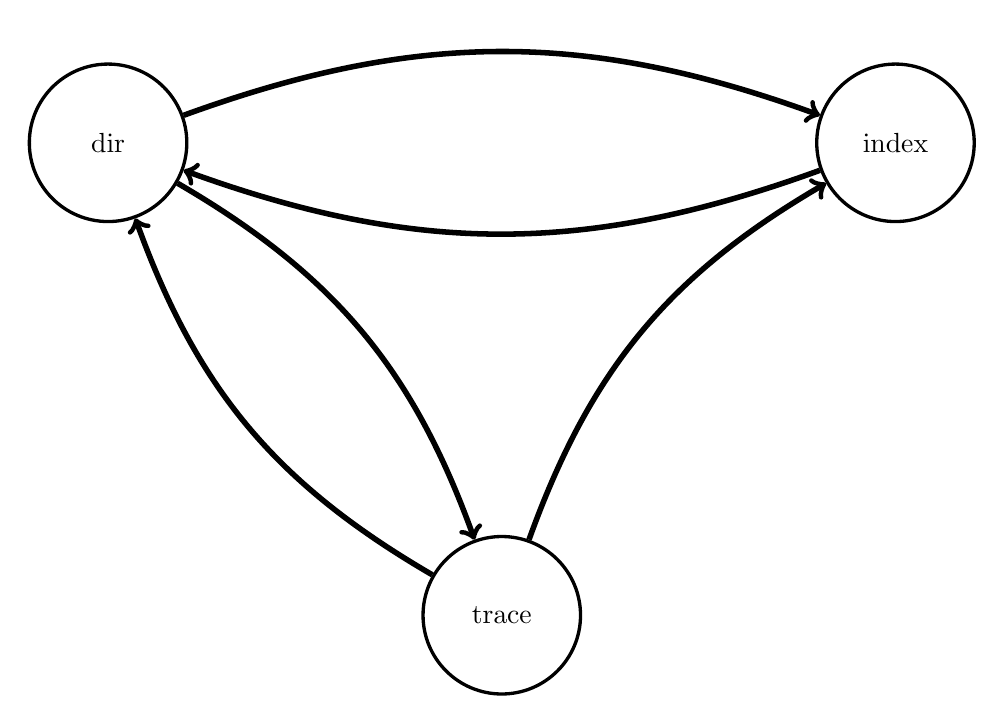
\begin{tikzpicture}[
    state/.style={draw = black, circle, minimum width = 2cm, very thick},
    arrow/.style={black, ->, line width = 2pt}
  ]
\begin{scope}[on grid]
\node[state] (dir)   {dir};
\node[state] (trace) [below right=6cm and 5cm of dir] {trace};
\node[state] (index) [right=10cm of dir] {index};
\end{scope}

\path (dir)   edge [arrow, bend right = -20] node [midway, above] {\gufidirindex}   (index);
\path (index) edge [arrow, bend left  =  20] node [midway, above] {\gufiindexdir}   (dir);

\path (dir)   edge [arrow, bend right = -20] node [midway, below] {\gufidirtrace}   (trace);
\path (trace) edge [arrow, bend left  =  20] node [midway, below] {\gufitracedir}   (dir);

\path (trace) edge [arrow, bend right = -20] node [midway, below] {\gufitraceindex} (index);
\end{tikzpicture}
\caption{Tools for Transforming Between Source Trees, Traces, and Indexes}
\end{figure}

\subsubsection{\gufitracedir}
\paragraph{Flags}
\begin{table} [H]
  \centering
  \begin{tabular}{l|l}
    Flag & Functionality \\
    \hline
    -h & help manual \\
    \hline
    -H & Show assigned input values \\
    \hline
    -v & version \\
    \hline
    -n \textless num\_threads\textgreater & define number of threads to use \\
    \hline
    -d \textless delim\textgreater & delimiter (one char)  [use 'x' for 0x1E] \\
    \hline
    -x & pull xattrs from source file-sys into GUFI \\
    \hline
  \end{tabular}
  \caption{\gufitracedir Flags and Arguments}
\end{table}

\paragraph{Usage} ~\\\\
\gufitracedir \texttt{[options] trace\_file... output\_dir}

\subsubsection{\gufiindexdir}
\paragraph{Flags}
\begin{table} [H]
  \centering
  \begin{tabular}{l|l}
    Flag & Functionality \\
    \hline
    -h & help manual \\
    \hline
    -H & Show assigned input values \\
    \hline
    -v & version \\
    \hline
    -n \textless num\_threads\textgreater & define number of threads to use \\
    \hline
    -x & pull xattrs from source file-sys into GUFI \\
    \hline
  \end{tabular}
  \caption{\gufiindexdir Flags and Arguments}
\end{table}

\paragraph{Usage} ~\\\\
\gufiindexdir \texttt{[options] input\_dir output\_dir}


% This file is part of GUFI, which is part of MarFS, which is released
% under the BSD license.
%
%
% Copyright (c) 2017, Los Alamos National Security (LANS), LLC
% All rights reserved.
%
% Redistribution and use in source and binary forms, with or without modification,
% are permitted provided that the following conditions are met:
%
% 1. Redistributions of source code must retain the above copyright notice, this
% list of conditions and the following disclaimer.
%
% 2. Redistributions in binary form must reproduce the above copyright notice,
% this list of conditions and the following disclaimer in the documentation and/or
% other materials provided with the distribution.
%
% 3. Neither the name of the copyright holder nor the names of its contributors
% may be used to endorse or promote products derived from this software without
% specific prior written permission.
%
% THIS SOFTWARE IS PROVIDED BY THE COPYRIGHT HOLDERS AND CONTRIBUTORS "AS IS" AND
% ANY EXPRESS OR IMPLIED WARRANTIES, INCLUDING, BUT NOT LIMITED TO, THE IMPLIED
% WARRANTIES OF MERCHANTABILITY AND FITNESS FOR A PARTICULAR PURPOSE ARE DISCLAIMED.
% IN NO EVENT SHALL THE COPYRIGHT HOLDER OR CONTRIBUTORS BE LIABLE FOR ANY DIRECT,
% INDIRECT, INCIDENTAL, SPECIAL, EXEMPLARY, OR CONSEQUENTIAL DAMAGES (INCLUDING,
% BUT NOT LIMITED TO, PROCUREMENT OF SUBSTITUTE GOODS OR SERVICES; LOSS OF USE,
% DATA, OR PROFITS; OR BUSINESS INTERRUPTION) HOWEVER CAUSED AND ON ANY THEORY OF
% LIABILITY, WHETHER IN CONTRACT, STRICT LIABILITY, OR TORT (INCLUDING NEGLIGENCE
% OR OTHERWISE) ARISING IN ANY WAY OUT OF THE USE OF THIS SOFTWARE, EVEN IF
% ADVISED OF THE POSSIBILITY OF SUCH DAMAGE.
%
%
% From Los Alamos National Security, LLC:
% LA-CC-15-039
%
% Copyright (c) 2017, Los Alamos National Security, LLC All rights reserved.
% Copyright 2017. Los Alamos National Security, LLC. This software was produced
% under U.S. Government contract DE-AC52-06NA25396 for Los Alamos National
% Laboratory (LANL), which is operated by Los Alamos National Security, LLC for
% the U.S. Department of Energy. The U.S. Government has rights to use,
% reproduce, and distribute this software.  NEITHER THE GOVERNMENT NOR LOS
% ALAMOS NATIONAL SECURITY, LLC MAKES ANY WARRANTY, EXPRESS OR IMPLIED, OR
% ASSUMES ANY LIABILITY FOR THE USE OF THIS SOFTWARE.  If software is
% modified to produce derivative works, such modified software should be
% clearly marked, so as not to confuse it with the version available from
% LANL.
%
% THIS SOFTWARE IS PROVIDED BY LOS ALAMOS NATIONAL SECURITY, LLC AND CONTRIBUTORS
% "AS IS" AND ANY EXPRESS OR IMPLIED WARRANTIES, INCLUDING, BUT NOT LIMITED TO,
% THE IMPLIED WARRANTIES OF MERCHANTABILITY AND FITNESS FOR A PARTICULAR PURPOSE
% ARE DISCLAIMED. IN NO EVENT SHALL LOS ALAMOS NATIONAL SECURITY, LLC OR
% CONTRIBUTORS BE LIABLE FOR ANY DIRECT, INDIRECT, INCIDENTAL, SPECIAL,
% EXEMPLARY, OR CONSEQUENTIAL DAMAGES (INCLUDING, BUT NOT LIMITED TO, PROCUREMENT
% OF SUBSTITUTE GOODS OR SERVICES; LOSS OF USE, DATA, OR PROFITS; OR BUSINESS
% INTERRUPTION) HOWEVER CAUSED AND ON ANY THEORY OF LIABILITY, WHETHER IN
% CONTRACT, STRICT LIABILITY, OR TORT (INCLUDING NEGLIGENCE OR OTHERWISE) ARISING
% IN ANY WAY OUT OF THE USE OF THIS SOFTWARE, EVEN IF ADVISED OF THE POSSIBILITY
% OF SUCH DAMAGE.



\section{Implementation Details}
In addition to glue code that combines the various well known
technologies used to implement GUFI, there exists in the codebase
several pieces of code, design decisions, and optimizations that have
made GUFI performant.

% This file is part of GUFI, which is part of MarFS, which is released
% under the BSD license.
%
%
% Copyright (c) 2017, Los Alamos National Security (LANS), LLC
% All rights reserved.
%
% Redistribution and use in source and binary forms, with or without modification,
% are permitted provided that the following conditions are met:
%
% 1. Redistributions of source code must retain the above copyright notice, this
% list of conditions and the following disclaimer.
%
% 2. Redistributions in binary form must reproduce the above copyright notice,
% this list of conditions and the following disclaimer in the documentation and/or
% other materials provided with the distribution.
%
% 3. Neither the name of the copyright holder nor the names of its contributors
% may be used to endorse or promote products derived from this software without
% specific prior written permission.
%
% THIS SOFTWARE IS PROVIDED BY THE COPYRIGHT HOLDERS AND CONTRIBUTORS "AS IS" AND
% ANY EXPRESS OR IMPLIED WARRANTIES, INCLUDING, BUT NOT LIMITED TO, THE IMPLIED
% WARRANTIES OF MERCHANTABILITY AND FITNESS FOR A PARTICULAR PURPOSE ARE DISCLAIMED.
% IN NO EVENT SHALL THE COPYRIGHT HOLDER OR CONTRIBUTORS BE LIABLE FOR ANY DIRECT,
% INDIRECT, INCIDENTAL, SPECIAL, EXEMPLARY, OR CONSEQUENTIAL DAMAGES (INCLUDING,
% BUT NOT LIMITED TO, PROCUREMENT OF SUBSTITUTE GOODS OR SERVICES; LOSS OF USE,
% DATA, OR PROFITS; OR BUSINESS INTERRUPTION) HOWEVER CAUSED AND ON ANY THEORY OF
% LIABILITY, WHETHER IN CONTRACT, STRICT LIABILITY, OR TORT (INCLUDING NEGLIGENCE
% OR OTHERWISE) ARISING IN ANY WAY OUT OF THE USE OF THIS SOFTWARE, EVEN IF
% ADVISED OF THE POSSIBILITY OF SUCH DAMAGE.
%
%
% From Los Alamos National Security, LLC:
% LA-CC-15-039
%
% Copyright (c) 2017, Los Alamos National Security, LLC All rights reserved.
% Copyright 2017. Los Alamos National Security, LLC. This software was produced
% under U.S. Government contract DE-AC52-06NA25396 for Los Alamos National
% Laboratory (LANL), which is operated by Los Alamos National Security, LLC for
% the U.S. Department of Energy. The U.S. Government has rights to use,
% reproduce, and distribute this software.  NEITHER THE GOVERNMENT NOR LOS
% ALAMOS NATIONAL SECURITY, LLC MAKES ANY WARRANTY, EXPRESS OR IMPLIED, OR
% ASSUMES ANY LIABILITY FOR THE USE OF THIS SOFTWARE.  If software is
% modified to produce derivative works, such modified software should be
% clearly marked, so as not to confuse it with the version available from
% LANL.
%
% THIS SOFTWARE IS PROVIDED BY LOS ALAMOS NATIONAL SECURITY, LLC AND CONTRIBUTORS
% "AS IS" AND ANY EXPRESS OR IMPLIED WARRANTIES, INCLUDING, BUT NOT LIMITED TO,
% THE IMPLIED WARRANTIES OF MERCHANTABILITY AND FITNESS FOR A PARTICULAR PURPOSE
% ARE DISCLAIMED. IN NO EVENT SHALL LOS ALAMOS NATIONAL SECURITY, LLC OR
% CONTRIBUTORS BE LIABLE FOR ANY DIRECT, INDIRECT, INCIDENTAL, SPECIAL,
% EXEMPLARY, OR CONSEQUENTIAL DAMAGES (INCLUDING, BUT NOT LIMITED TO, PROCUREMENT
% OF SUBSTITUTE GOODS OR SERVICES; LOSS OF USE, DATA, OR PROFITS; OR BUSINESS
% INTERRUPTION) HOWEVER CAUSED AND ON ANY THEORY OF LIABILITY, WHETHER IN
% CONTRACT, STRICT LIABILITY, OR TORT (INCLUDING NEGLIGENCE OR OTHERWISE) ARISING
% IN ANY WAY OUT OF THE USE OF THIS SOFTWARE, EVEN IF ADVISED OF THE POSSIBILITY
% OF SUCH DAMAGE.



\subsection{\qptp}
Thread pools are generally written with a single work thread (with a
single lock) from which to threads pull from. This does not work past
a handful of threads. GUFI can run on hundreds of threads, and thus
required a more performant thread pool. The solution to this was
\qptp.

\qptp is named so because originally, there was one work queue (and
lock) maintained for each thread in the thread pool. Now, there are
multiple work queues maintained for each thread: work is pushed to the
waiting work queue and the claimed work queue contains the work that
the thread claimed for processing.

\subsubsection{Adding Work}
By default, work is added to threads in a round robin fashion in order
to distribute work evenly and to attempt to prevent, or at least
reduce the amount of, contention experienced by any one work queue.

This function can be changed during initialization.

\subsubsection{Processing Queued Work}
Because work items are enqueued in parallel while work items are
processed, popping off work items one at a time results in one lock
per removal that might experience contention while the queue is being
modified. In \qptp, when a thread claims (pops off) work for
processing, {\bf all} work items in the waiting work queue are moved
to the claimed work queue, resulting in the removal of multiple work
items with only a single lock that might experience contention. All
claimed work is processed before the thread returns to the work queue
to find more work.

If a thread discovers that it does not have work items in its waiting
work queue but the thread pool still has outstanding in-memory work,
it will search for more work in the waiting queue of other threads. If
work items are found, the thread will steal at least one item, causing
the stolen work items to experience less latency between enqueuing and
processing. If no work can be stolen from the waiting work queues of
all threads, the thread will attempt to take work from the claimed
work queue. This is done so that long running jobs do not prevent
claimed work from being processed. This also makes \qptp behave more
like thread pools that pull one work item off at a time and thus
always processes work when work is available.

If the queue size limit was set before the thread pool was started and
a thread's work item count is greater than or equal to the queue size
limit, new work items are swapped to a filesystem instead of cached in
memory. These work items are not counted as in-memory outstanding
work, and are instead processed after all in-memory work items have
been processed, in \texttt{QPTPool\_wait}. This should be considered a
last-ditch attempt to prevent OOM-ing, and should not occur too often.

\subsubsection{Usage}
\begin{enumerate}
\item Create a thread pool:

  \texttt{QPTPool\_t *pool = QPTPool\_init(nthreads, args);}

  \texttt{nthreads} sets the number of threads in this thread
  pool.

  The \texttt{args} argument will be accessible by all threads that
  are run.

\item Setting Properties:

  \texttt{QPTPool\_init} is intentionally kept simple and uses default
  values for some features. These values may be modified using
  \texttt{QPTPool\_init\_with\_props} or \texttt{QPTPool\_set\_*}
  functions before \texttt{QPTPool\_start} is called.

  By default, \qptp will push new work items in a round robin
  fashion. This can be changed to a custom function with
  \\\texttt{QPTPool\_set\_next}. This function is set at the context
  level instead of at \texttt{QPTPool\_enqueue} in order to not
  require a branch to figure out whether or not the provided function
  pointer is valid.

  \texttt{QPTPool\_set\_queue\_limit} causes work items to be swapped
  to a filesystem.

  \texttt{QPTPool\_set\_swap\_prefix} sets the path where swap data is
  written. Note that this prefix is prefixed to the path string
  directly, without a path separator. Additionally, the parent
  directory of the prefix must already exist - the path is not created
  if it does not exist.

  \texttt{QPTPool\_set\_steal} sets the numerator and denominator of
  the multiplier used when work items are being stolen from other
  threads. If the queue being inspected has at least one work item on
  it, \texttt{max(queue.size * numerator / denominator, 1)} work items
  are taken from the front of the queue.

\item Getting Properties:

  Properties may be extracted from the context using the
  \texttt{QPTPool\_get\_*} functions.

\item Start the thread pool:

  \texttt{QPTPool\_start(pool);}

\item Add work:

  \begin{itemize}
    \item \texttt{QPTPool\_enqueue(pool, id, function, work);}

    The function passed into \texttt{QPTPool\_enqueue} must match the
    signature found in \texttt{QueuePerThreadPool.h}. The
    \texttt{work} argument will only be accessible to the thread
    processing this work.

    The thread that will receive the new work item is not \texttt{id}.
    Rather, \texttt{id} is treated as the source thread id and
    \texttt{threads[id]->next\_queue} will be where the new work item
    is enqueued.

    Work enqueued with \texttt{QPTPool\_enqueue} will not be swapped.

    \item \texttt{QPTPool\_enqueue\_swappable(pool, id, func, work, serialize, deserialize);}

    Work passed into \texttt{QPTPool\_enqueue\_swappable} may end up
    in the wait queue or be swapped to a filesystem.

    The thread that will receive the new work item is not \texttt{id}.
    Rather, \texttt{id} is treated as the source thread id and
    \texttt{threads[id]->next\_queue} will be where the new work item
    is enqueued.

    \item \texttt{QPTPool\_enqueue\_here(pool, id, queue, func, work, serialize, deserialize);}

    If the queue argument is set to \texttt{QPTPool\_enqueue\_WAIT},
    the work will be explicitly placed into the selected queue at
    thread \texttt{id} instead of using the next thread selection
    function. The queue limit is ignored.

    If the queue argument is set to \texttt{QPTPool\_enqueue\_SWAP},
    the work will be written to the selected thread's swap space.
  \end{itemize}

\item Wait for work to be completed (optional):

  \begin{itemize}
    \item \texttt{QPTPool\_wait\_mem\_lte(pool, count);}

      This function waits until the amount of in-memory work to be
      done is less than or equal to \texttt{count}.

    \item \texttt{QPTPool\_wait\_mem(pool);}

      This function waits until all in-memory work to be done. This
      function is just \texttt{QPTPool\_wait\_mem\_lte(pool, 0);}

    \item \texttt{QPTPool\_wait(pool);}

      This function waits until all in-memory and swapped work is done.
  \end{itemize}

\item Wait for all work to be completed (threads are joined):

  \texttt{QPTPool\_stop(pool);}

  This function exists to allow for the collection of statistics
  before the context is destroyed. Note that \texttt{QPTPool\_wait} is
  called by this function, and thus does not have to be explicitly
  called before calling this function.

\item Destroy the pool context:

  \texttt{QPTPool\_destroy(pool);}
\end{enumerate}

\input{sections/bottomup}
\input{sections/printing}
% This file is part of GUFI, which is part of MarFS, which is released
% under the BSD license.
%
%
% Copyright (c) 2017, Los Alamos National Security (LANS), LLC
% All rights reserved.
%
% Redistribution and use in source and binary forms, with or without modification,
% are permitted provided that the following conditions are met:
%
% 1. Redistributions of source code must retain the above copyright notice, this
% list of conditions and the following disclaimer.
%
% 2. Redistributions in binary form must reproduce the above copyright notice,
% this list of conditions and the following disclaimer in the documentation and/or
% other materials provided with the distribution.
%
% 3. Neither the name of the copyright holder nor the names of its contributors
% may be used to endorse or promote products derived from this software without
% specific prior written permission.
%
% THIS SOFTWARE IS PROVIDED BY THE COPYRIGHT HOLDERS AND CONTRIBUTORS "AS IS" AND
% ANY EXPRESS OR IMPLIED WARRANTIES, INCLUDING, BUT NOT LIMITED TO, THE IMPLIED
% WARRANTIES OF MERCHANTABILITY AND FITNESS FOR A PARTICULAR PURPOSE ARE DISCLAIMED.
% IN NO EVENT SHALL THE COPYRIGHT HOLDER OR CONTRIBUTORS BE LIABLE FOR ANY DIRECT,
% INDIRECT, INCIDENTAL, SPECIAL, EXEMPLARY, OR CONSEQUENTIAL DAMAGES (INCLUDING,
% BUT NOT LIMITED TO, PROCUREMENT OF SUBSTITUTE GOODS OR SERVICES; LOSS OF USE,
% DATA, OR PROFITS; OR BUSINESS INTERRUPTION) HOWEVER CAUSED AND ON ANY THEORY OF
% LIABILITY, WHETHER IN CONTRACT, STRICT LIABILITY, OR TORT (INCLUDING NEGLIGENCE
% OR OTHERWISE) ARISING IN ANY WAY OUT OF THE USE OF THIS SOFTWARE, EVEN IF
% ADVISED OF THE POSSIBILITY OF SUCH DAMAGE.
%
%
% From Los Alamos National Security, LLC:
% LA-CC-15-039
%
% Copyright (c) 2017, Los Alamos National Security, LLC All rights reserved.
% Copyright 2017. Los Alamos National Security, LLC. This software was produced
% under U.S. Government contract DE-AC52-06NA25396 for Los Alamos National
% Laboratory (LANL), which is operated by Los Alamos National Security, LLC for
% the U.S. Department of Energy. The U.S. Government has rights to use,
% reproduce, and distribute this software.  NEITHER THE GOVERNMENT NOR LOS
% ALAMOS NATIONAL SECURITY, LLC MAKES ANY WARRANTY, EXPRESS OR IMPLIED, OR
% ASSUMES ANY LIABILITY FOR THE USE OF THIS SOFTWARE.  If software is
% modified to produce derivative works, such modified software should be
% clearly marked, so as not to confuse it with the version available from
% LANL.
%
% THIS SOFTWARE IS PROVIDED BY LOS ALAMOS NATIONAL SECURITY, LLC AND CONTRIBUTORS
% "AS IS" AND ANY EXPRESS OR IMPLIED WARRANTIES, INCLUDING, BUT NOT LIMITED TO,
% THE IMPLIED WARRANTIES OF MERCHANTABILITY AND FITNESS FOR A PARTICULAR PURPOSE
% ARE DISCLAIMED. IN NO EVENT SHALL LOS ALAMOS NATIONAL SECURITY, LLC OR
% CONTRIBUTORS BE LIABLE FOR ANY DIRECT, INDIRECT, INCIDENTAL, SPECIAL,
% EXEMPLARY, OR CONSEQUENTIAL DAMAGES (INCLUDING, BUT NOT LIMITED TO, PROCUREMENT
% OF SUBSTITUTE GOODS OR SERVICES; LOSS OF USE, DATA, OR PROFITS; OR BUSINESS
% INTERRUPTION) HOWEVER CAUSED AND ON ANY THEORY OF LIABILITY, WHETHER IN
% CONTRACT, STRICT LIABILITY, OR TORT (INCLUDING NEGLIGENCE OR OTHERWISE) ARISING
% IN ANY WAY OUT OF THE USE OF THIS SOFTWARE, EVEN IF ADVISED OF THE POSSIBILITY
% OF SUCH DAMAGE.



\subsection{Optimizations}
In order for GUFI to be performant, many optimizations were used and
implemented.

\subsubsection{Reduced Branching}
In order to reduce the number of failed branch predictions experienced
by GUFI, branching was removed where possible. The main way this was
done was by intentionally skipping \texttt{NULL} pointer checks that
are repeated or always expected to be valid.

\subsubsection{Allocations}
Allocations are not performed by the standard malloc. Instead,
\texttt{jemalloc(3)} is used to override \texttt{malloc(3)}. See
\href{https://jemalloc.net/}{jemalloc's website} for details.

\subsubsection{Not Calling \lstat During Tree Walk}
\texttt{struct~dirent}s are returned when reading a directory with
\readdir. glibc's implementation of \texttt{struct~dirent} provides
extra fields not required by POSIX.1. GUFI takes advantage of the
nonstandard \texttt{d\_type} field to not call \lstat when determining
whether or not the entry is a directory. Only when \texttt{d\_type} is
not set will \lstat be called.

\subsubsection{Enqueuing Work Before Processing}
In order to reduce the amount of time the thread pool spends waiting
for work, work is enqueued before doing the main processing for a
directory. When walking a tree, such as with \gufidirindex,
\gufidirtrace, and \gufiquery, subdirectories are enqueued before
processing source filesystem information and running
queries. \gufitraceindex reads each trace file using a single
thread. However, each stanza is not processed as it is
encountered. Instead, each stanza's file offset is enqueued in the
thread pool, allowing for the directories of the index to be generated
in parallel.

\subsubsection{String Manipulations}
Where possible, strings are not copied, and are instead referenced.
Additionally, calls to \texttt{strlen(3)} are avoided in order to not
walk memory one byte at a time. Some string lengths, such as those for
input arguments are obtained with \texttt{strlen(3)}. Afterwards,
string manipulations are done by using or modifying lengths to offset
into or cut short strings.

\subsubsection{Combining Strings with \memcpy}
One method of combining C-strings is by concantenating them with
\texttt{snprintf(3)} with format strings containing only \texttt{\%s}
format specifiers. Instead of parsing the format string, the
\texttt{SNFORMAT\_S} function was created to do \memcpy s on the
arguments, skipping figuring out whether or not inputs are strings and
how long they are by finding \texttt{NULL} terminators. Instead,
lengths are obtained as by-products of previous string manipulations
and the values are reused.

\subsubsection{In-Situ Processing}
Occassionally, GUFI might encounter extremely large directories. This
results in many long lived dynamic allocations being created during
descent, which can overwhelm memory. Users can set a subdirectory
limit so that if too many subdirectories are encountered within a
single directory, subdirectories past the user provided count will be
processed recursively using a work item allocated on the thread's
stack instead of being dynamically allocated and enqueued for
processing. This reduces memory pressure by limiting the amount of
work items that extremely large directories would otherwise spawn. The
subdirectories being processed recursively may themselves enqueue
dynamically allocated subdirectory work or recurse further down with
subdirectory work allocated on the stack.

\subsubsection{Smaller Enqueued Work Items}
The main data structure that is enqueued is \work. This
struct started at approximately 14KiB in size.

\href{https://github.com/mar-file-system/GUFI/commit/2227d00665eb6d507ac2052e80616c077a5da853}{2227d00}
moved the parts of this structure that were not necssary for directory
tree traversal to \texttt{struct~entry\_data}, reducing
\work to slightly over 8KiB. This was used to fix
\href{https://github.com/mar-file-system/GUFI/issues/121}{Issue~121}.

\href{https://github.com/mar-file-system/GUFI/commit/e260d26aab0713835defbe2a5b6e1187610dcf3d}{e260d26}
changed \work so that the name field was a flexible
array stored after the other struct members, reducing
\work down to $\sim$200~bytes (depends on the length of the
path). However, C++ does not support flexible arrays, so
\href{https://github.com/mar-file-system/GUFI/commit/d1265f9ee9a5aa4451400f5abb455eb3ad64957c}{d1265f9}
was pushed, returning the \texttt{name} member back to its original
position, but making it a pointer that points to a location after the
struct.

\subsubsection{Compression with zlib}
When zlib is detected during CMake configuration, \work can be
compressed to further reduce the size of each work item that is
sitting in memory waiting to be processed. The compressed buffer,
originally allocated with
\texttt{sizeof(struct~work)~+~name\_len~+~1)} bytes, is then
reallocated to the compressed size. The bulk of \work is made up of
text strings followed by \texttt{NULL} characters, both of which are
highly compressible, meaning that compressed work items can be
expected to be much smaller than uncompressed work items.

Note that \work is its own compressed buffer. Whether
or not the work item is compressed and the compressed length are now
the first two fields of \work. When a work item is
compressed, a pointer pointing to it will have less space allocated to
it than \texttt{sizeof(struct~work)~+~name\_len~+~1)}.

This was used to fix
\href{https://github.com/mar-file-system/GUFI/issues/121}{Issue 121}.

\subsubsection{Database Templates}
Every directory in an index contains at least one database file,
called db.db, containing the \lstat data from the source
filesystem. When creating indexes, a database file is created with
the same schema as db.db and is left unfilled. When each directory in
the index is processed, the database file created earlier is copied
into the directory as a bytestream instead of having SQlite open new
database files for each directory. This avoids the multitudes of
checks done by SQLite when setting up databases and tables. The same
is done for external xattr database files.

\subsubsection{SQLite}
As SQLite is a major component in GUFI, attempts were made to optimize
its usage. Some optimizations were made at compile time. See the
\href{https://www.sqlite.org/compile.html}{SQLite Compile-time
  Options} page for details.

\paragraph{Locking}
In order to prevent multiple threads from corrupting data, SQLite
implements locking. In GUFI, each database is only ever accessed by
one thread:

\begin{itemize}
\item When indexing, only one thread writes to each directory's
  database.
\item When querying, the per-thread results are written to per-thread
  databases. After the tree walk, the per-thread databases are merged
  serially into a final database.
\end{itemize}

Locking despite never modifying databases in parallel is not useful,
and was removed by setting \texttt{-DSQLITE\_THREADSAFE=0} in the
compile flags.

\paragraph{VFS}
In addition to not locking SQLite in-memory operations, locking at the
filesystem level was also disabled. Instead of opening SQLite database
files with the default VFS, GUFI uses the \texttt{unix-none} VFS,
which causes all file locking to become no-ops. See
\href{https://www.sqlite.org/vfs.html}{The SQLite OS Interface or
 ``VFS''} for details.

\paragraph{Memory Tracking}
Memory tracking was disabled with \\
\noindent \texttt{-DSQLITE\_DEFAULT\_MEMSTATUS=0}.

\paragraph{Temporary Files}
Temporary files can be stored to disk or in memory. GUFI forces all
temporary files to be stored in memory with \\
\texttt{-DSQLITE\_TEMP\_STORE=3}.

\subsubsection{Caching Queries (Not Merged)}
When queries are performed on indexes, they are processed from
scratch by each thread for each directory. An obvious optimization
would be to reduce the amount of string parsing and query planning by
compiling each query once (or a small number of times such as once per
thread) at the beginning of a run and saving the compiled queries for
repeated use during the index traversal.

An attempt at caching queries was made with
\href{https://github.com/mar-file-system/GUFI/pull/95}{Pull~Request~\#95}.
Unfortunately, caching queries at best seemed to perform on par with
the latest GUFI and at worst, slightly slower than the latest
GUFI. This was true for both simple queries and complex queries with
\texttt{JOIN}s.



\end{document}
